
% common/newnames.tex & common/renames.tex
{\actuality} Биологические модели занимают важное место в теории динамических систем, охватывая широкий спектр явлений, происходящих в биологических процессах. Эти модели включают как те, которые описывают концентрацию различных веществ в биологических системах, таких как химические реакции в клетках или процессы обмена веществ в организмах, так и популяционные уравнения, моделирующие изменение численности и структуру популяций живых существ. Обычно модели популяционной динамики описываются дифференциальными или дифференциально-разностными уравнениями. 
Эти модели с течением времени претерпели значительные изменения и усложнения.

Одной из первых популяционных моделей была модель Томаса Мальтуса, который предположил, что рост популяции, не сдерживаемой ограничениями на ресурсы, будет экспоненциальным. Массовые вымирания, такие как эпидемии, голод и войны, в модели Мальтуса объясняются тем, что ресурсы, необходимые для выживания, не могут воспроизводиться с такой же скоростью, как и популяция, что приводит к перенаселению \cite{Malthus1798}.

Пьер Ферхюльст в работе \cite{Verhulst1838} предложил добавить в модель Мальтуса квадратичное слагаемое, ограничивающее скорость роста популяции для больших значений её размера. Таким образом, он получил модель, называемую логистическим уравнением
\begin{equation}
\label{eq:intro:logistic}
	\dot{x}=\lambda x\left(1-\frac{x}{K}\right),
\end{equation}
где функция $x(t)$ показывает текущую плотность (или численность) популяции, параметр $\lambda$ характеризует скорость роста популяции, а параметр $K$ --- ёмкость среды.

Позже рассматривались различные усовершенствования приведённой модели. Одна из идей усложнения правой части уравнения \eqref{eq:intro:logistic} --- добавление запаздывания. Так в 1948 году Джордж Хатчинсон предложил модификацию логистического уравнения, обладающую запаздыванием по времени и простейшим образом учитывающую возрастную структуру популяции:
%
\begin{equation}
\label{eq:intro:hutch}
	\dot{x}=\lambda x\left(1 - \frac{x(t-\tau)}{K}\right),
\end{equation}
%
где $x(t)$ --- плотность популяции, $\lambda$ --- скорость роста популяции, $K$ --- ёмкость среды, запаздывание $\tau$ --- возраст половозрелости \cite{Hutchinson1948}. %https://encyclopediaofmath.org/wiki/Hutchinson_equation

Помимо уравнения Хатчинсона, рассматривались различные его обобщения с заменой квадратичной зависимости в правой части на более сложную. Например, в работе \cite{Glyzin2007} предлагается модель, более тонко учитывающая возрастную структуру
\begin{equation}
	\dot{x}=\lambda \left(1 - \frac{1}{K}\sum\limits_{i = 1}^{m} a_i x(t-\tau_i)\right) x.
\end{equation}
%
В работе \cite{Kaschenko2012} исследуется обобщение модели с непрерывным запаздыванием
\begin{equation}
	\dot{x} = \lambda \left(1 - \int\limits_{h_1}^{h_2}dr(\tau)x(t - \tau)\right) x,
\end{equation}
где $r(\tau)$ --- монотонная неотрицательная функция, $\lambda, h_1, h_2$ --- положительные параметры.

В работе \cite{Kolesov2010} предлагается обобщение модели, определённое уравнением
\begin{equation}
\label{eq:intro:hutch_modified}
	\dot{x} = \lambda f(x(t - 1)) x,
\end{equation}
%
где бесконечно дифференцируемая при $t \geq 0$ функция $f$ обладает свойствами
\[
f(0) = 1, \quad f(x) = -a_0 + \sum\limits_{k = 1}^{\infty} \frac{a_k}{x^k}, \quad x \to +\infty, \quad a_0 > 0.
\]
После экспоненциальной замены $x = e^{\lambda y}$ уравнение \eqref{eq:intro:hutch_modified} принимает вид
\begin{equation}
\label{eq:intro:hutch_modified_exp}
\dot{y} = f(e^{\lambda y(t - 1)}).
\end{equation}
При достаточно большом $\lambda$ правая часть становится близкой к релейной функции, меняющей значение при смене знака аргумента.

Типичным примером такой функции служит
\[
f(x) = \dfrac{1 - x}{1 + cx}, \quad c = \text{const} > 0.
\]
В работе \cite{Kolesov2010} отмечается, что при больших значениях параметра $\lambda$ уравнение \eqref{eq:intro:hutch_modified} обладает лучшими биологическими характеристиками, чем уравнение \eqref{eq:intro:hutch}: это связано с тем, что решение уравнения \eqref{eq:intro:hutch} обладает очень глубоким минимумом, который в биологическом контексте означает вымирание популяции после первого же всплеска численности (см. рис. \ref{fig:intro:hutch}).

%\fixme{Отметим, что в отличие от модели Мальтуса, модель \eqref{eq:intro:logistic} и все перечисленные её обобщения обладают насыщением, т.е. плотность популяции, характеризуемая функцией $x(t)$, ограничена сверху.}

\fixme{Это корректно?}

\fixme{Отметим, что приведённые выше модели \eqref{eq:intro:logistic} -- \eqref{eq:intro:hutch_modified} обладают характерными для популяционных моделей <<вольтерровского типа>> свойствами. Так, решение с положительными начальными условиями остаётся положительным при $t > 0$; модели имеют положительное состояние равновесия, соответствующее ёмкости среды.}

\fixme{Однако, уравнение \eqref{eq:intro:hutch_modified} является моделью с насыщением, т.~е., как видно из уравнения \eqref{eq:intro:hutch_modified_exp}, любое решение ограничено константой, не зависящей от параметра $\lambda$.}
	
\begin{figure}
	\centering
	\includegraphics[width=0.7\textwidth]{hutch.png}
	\caption{Слева: решение уравнения \eqref{eq:intro:hutch} при $\lambda = 2.5$, $K = 1$, $\tau = 1$; справа: решение уравнения \eqref{eq:intro:hutch_modified} при $\lambda = 2.5$, $c = 0.2$. Решение (а) обладает близким к нулю минимумом, что в биологическом контексте означает полное вымирание популяции; у решения (б) этот недостаток отсутствует.\\Иллюстрация взята из статьи \cite{Kolesov2010}.}
	\label{fig:intro:hutch}
\end{figure}

Нелинейности, представленные рациональными функциями, также встречаются в различных биологических системах, включая генные сети, которые будут рассмотрены позже. Одним из примеров таких систем является модель Мэки--Гласса, исследуемая в данной диссертационной работе.

Уравнениями Мэки--Гласса называют две модели с запаздыванием \cite{Mackey1977, Glass1988}:
\begin{equation}
	\label{eq:mg_equation_1:intro}
	\dot{v}=-b v+\frac{a \theta^{\gamma} v(t-\tau)}{\theta^{\gamma}+(v(t-\tau))^{\gamma}},
\end{equation}
\begin{equation}
	\label{eq:mg_equation_2:intro}
	\dot{v}=-b v+\frac{a \theta^{\gamma}}{\theta^{\gamma}+(v(t-\tau))^{\gamma}},
\end{equation}
где параметры $a, b, \gamma, \theta$ --- положительные вещественные числа.

Эти модели были предложены в работе \cite{Mackey1977} для описания регуляторных функций в процессах кроветворения. Уравнения \eqref{eq:mg_equation_1:intro} и \eqref{eq:mg_equation_2:intro} различаются формой нелинейности в слагаемом с запаздыванием: в уравнении \eqref{eq:mg_equation_2:intro} она монотонно убывает, в то время как в уравнении \eqref{eq:mg_equation_1:intro} имеет форму <<горба>>. В данной работе под уравнением Мэки--Гласса будет пониматься уравнение \eqref{eq:mg_equation_1:intro}.

Биологический смысл данной модели следующий: функция $v(t)$ --- плотность циркулирующих в крови человека нейтрофилов (вид лейкоцитов) в клетках на кг массы тела, $b$ --- скорость случайного распада нейтрофилов, положительное слагаемое означает текущий приток клеток в кровь, возникающий в ответ на запрос, создавшийся в некоторый момент $\tau$ в прошлом.

В широком диапазоне изменений уровня циркулирующих нейтрофилов скорость образования нейтрофилов падает с увеличением их плотности. Однако благодаря действию различных факторов можно ожидать, что при очень низких уровнях нейтрофилов скорость их образования будет падать, приближаясь к нулю \cite[с. 85]{Mackey1977}. Форма нелинейности выбирается из приведённых соображений.

Уравнение Мэки--Гласса исследовалось во множестве работ: например, см. \cite{Junges2012, Su2011, Wu2007, Kubyshkin2016, Krisztin2020, Bartha2021}. В оригинальной работе \cite{Mackey1977} приведены численные решения, как в случае периодических, так и непериодических колебаний. В работах \cite{Krisztin2020, Bartha2021} исследуются периодические решения уравнения Мэки--Гласса. В частности, в \cite{Bartha2021} доказано (при некоторых ограничениях на параметры и множество начальных функций) существование и единственность орбитально устойчивого предельного цикла.

Уравнение допускает различные обобщения. Так, в работе \cite{Berezansky2006} исследуется аналог уравнения Мэки--Гласса с переменным запаздыванием. В работе \cite{Liz2002} изучаются асимптотические свойства решений уравнений <<типа Мэки--Гласса>> с нелинейностью похожей формы. В \cite{Huang2024} изучается стохастическая версия уравнения с несколькими запаздываниями. В статье \cite{Berezansky2012} представлен обширный обзор различных известных (к 2012 г.) результаты, связанные с исследованием уравнения Мэки--Гласса и его обобщений, со ссылками на соответствующие работы.

Уравнение Мэки--Гласса и его различные модификации широко использовались для моделирования функционирования электрогенераторов \cite{Tateno2012, Namajunas1995, Glyzin2018, Glyzin2018a}, а также для симуляции хаотического сигнала \cite{Grassberger1983, Amil2015, Amil2015a, Shahverdiev2006}.

Помимо биологических моделей, описываемых одним уравнением, представляют интерес модели, получаемые объединением элементов, функционирующих некоторым известным образом, в сеть. Следует отметить, что цепочки идентичных нелинейных осцилляторов используются в качестве математических моделей в различных областях естествознания: биофизике, экологии, оптике, химической кинетике, нейродинамике, генной инженерии и др. \cite{Glyzin2022}. Можно выделить две естественные структуры для связи элементов сети: кольцо, где элемент связан с соседними элементами, и полносвязную сеть (рис. \ref{fig:full_mesh:intro}), где каждый элемент цепи связан со всеми остальными.

\begin{figure}[ht]
	\centering
	\includegraphics[width=0.5\textwidth]{mg_generator_full.eps}
	\caption{Полносвязная цепь осцилляторов. Каждый осциллятор является передающим и принимающим для всех остальных осцилляторов в цепи.}
	\label{fig:full_mesh:intro}
\end{figure}

Примером такой системы являются искусственные генные сети. Интерес к искусственным генным осцилляторам вызван тем обстоятельством, что они являются упрощёнными моделями таких ключевых биологических процессов, как клеточный цикл и циркадные ритмы. Простейший генетический осциллятор, предложенный в \cite{Elowitz2000} и названный репрессилятором, состоит как минимум из трёх элементов, соединённых в кольцо \cite{GlyzinBook2018}. Функционирование такой сети описывается системой
\begin{equation}
	\label{eq:intro:repressilator}
	\dot{u}_j = -u_j + \dfrac{\alpha}{1 + u^{\gamma}_{j - 1}}, \quad j = 1, 2, 3,
\end{equation}
где $u_0 = u_3$, $\alpha, \gamma > 0$. Исследование генных сетей проводится в работах \cite{Likhoshvaj2003, Volokitin2004, Golubyatnikov2006, Buse2009, Buse2010}.

Аналогичным образом можно соединить в цепь элементы, функционирование которых описывается уравнением \eqref{eq:mg_equation_1:intro}. Такие системы были исследованы во множестве работ \cite{Preobrazhenskaia2021, Tateno2012, Sano2007, Wan2009}. Так, в \cite{Sano2007} численно и экспериментально изучалась система из четырёх генераторов Мэки--Гласса, два из которых были вещательными, а два --- принимающими. В работе \cite{Wan2009} исследовалась потеря устойчивости состояния равновесия в этой системе, а также условия, при которых в результате бифуркации рождается устойчивый предельный цикл.

В диссертационной работе методами большого параметра исследуются периодические режимы, возникающие в полносвязной цепи осцилляторов, функционирование которых описывается уравнением Мэки--Гласса. Доказывается существование периодических режимов специального вида: дискретных бегущих волн и двухкластерной синхронизации, описание которых даётся ниже.

{\methods} Для сложных моделей в случае, когда не удается отыскать решение непосредственным интегрированием, уместно использование специальных методов поиска решения. В частности, это относится к дифференциальным уравнениям с запаздывающим аргументом. Одна из идей упрощения исследования --- это переход к предельному объекту.

Для упрощения исследования необходимо подобрать такую замену, чтобы при стремлении большого параметра $\gamma \to +\infty$ получилось релейное уравнение, у которого, с одной стороны, имеется достаточно сложная динамика (периодические решения различной структуры), а с другой стороны, при стремлении $\gamma \to +\infty$ можно было доказать сходимость решения исходного уравнения к периодическому решению релейной задачи. В частности, это получается сделать, если нелинейность в правой части уравнения близка к сигмоидальной функции, например, имеет вид $f_\gamma(u)=\frac{1}{1 + u^\gamma}$, $u > 0$ (см., например, \cite{Preobrazhenskaya2020, Glyzin2017, Krisztin2020, Bartha2021}). Такая функция в пределе при $\gamma\to+\infty$ устремляется к кусочно-постоянной функции, меняющей значение в 1. Тогда исходное уравнение можно заменить релейным, которое, как правило, существенно проще для анализа. После построения решения предельного уравнения доказывается существование асимптотически близкого решения исходной задачи.

Другая идея состоит в том, чтобы найти решение в специальном виде. Остановимся на описании этой процедуры подробнее.

%\textit{Переход к предельному объекту.} В ряде случаев при исследовании сложного уравнения удается определить содержательный предельный объект при устремлении одного из параметров к бесконечности (см., например, \cite{Kolesov1997}). В частности, это получается сделать, если нелинейность в правой части уравнения близка к сигмоидальной функции, например, имеет вид $f_\gamma(u)=\frac{1}{1 + u^\gamma}$, $u > 0$ (см., например, \cite{Preobrazhenskaya2020, Glyzin2017, Krisztin2020, Bartha2021}). Такая функция в пределе при $\gamma\to+\infty$ устремляется к кусочно-постоянной функции, меняющей значение в 1. Тогда исходное уравнение можно подменить релейным, которое, как правило, существенно проще для анализа. После построения решения предельного уравнения можно попытаться доказать существование асимптотически близкого решения исходной задачи.

\textit{Поиск решений специального вида.} В настоящей работе используются два подхода к построению специальных решений системы дифференциально-разностных уравнений, разработанные в работах С. Д. Глызина и др. \cite{GlyKol2013, GlyKol2013a, Glyzin2014}: это построение дискретных бегущих волн (вторая глава диссертации) и поиск режимов кластерной синхронизации (третья глава диссертации). Опишем метод построения решений того и другого сорта в общем виде.

\textit{Дискретные бегущие волны.} Рассмотрим симметричную систему осцилляторов, связанных либо в кольцо, либо в полносвязную систему. Дискретной бегущей волной называют периодическое решение, все компоненты которого представлены одной и той же периодической функцией $u(t)$ со сдвигом по времени, кратным некоторому параметру $\Delta$.

% Таким образом, решение представляется в следующем виде:

Для полносвязной сети релейных генераторов Мэки--Гласса, рассматриваемой во второй главе диссертации, соответствующая система имеет вид
%
\begin{equation}
	\label{eq:intro:mg_full_renormed}
	\dot{u}_j(t) = -\beta u_j(t) + \alpha F \left(u_j(t - 1) + \sum\limits_{k = 0, k\neq j}^m u_k(t)\right), \text{ где }
\end{equation}
\[
F(x) = \begin{cases}
	x, & x < 1;\\
	1/2, & x = 1;\\
	0, & x > 1.
\end{cases}
\]

После подстановки $u_j(t) = u(t + j\Delta)$ в систему \eqref{eq:intro:mg_full_renormed} получаем вспомогательное уравнение

\begin{equation}
	\label{eq:intro:mg_auxiliary}
	\dot{u}=-\beta u + \alpha F\left(\sum_{s=1}^{m}u(t-s\Delta)\right).
\end{equation}

Дискретной бегущей волне соответствует периодическое решение уравнения \eqref{eq:intro:mg_auxiliary}, период (не обязательно главный) которого кратен параметру $\Delta$. Отметим, что из существования одного решения в виде дискретной бегущей волны следует одновременное существование сразу $n!$ таких режимов, получаемых перестановкой компонент исходного решения, где $n$ --- количество уравнений в системе.


%Дискретные бегущие волны в кольцевых системах описаны в работах \cite{GlyKol2013a, Glyzin2016, Kolesov2016}, а в полносвязных --- в работах \cite{Glyzin2022, Glyzin2022a, Preobrazhenskii2024}.
%
%Пусть $n$ осцилляторов $x_1, \ldots, x_n$ описываются симметричной кольцевой системой дифференциальных уравнений
%\begin{equation}
%\label{eq:intro:sys_Phi_circ}
%	\dot{x}_j=\Phi(x_j, x_{j-1}), \quad j=1, \ldots, n, \quad x_{0} = x_{n},
%\end{equation}
%где $\Phi:\mathbb{R}^2\to\mathbb{R}$. 
%
%Дискретной бегущей волной называют периодическое решение, все компоненты которого представлены одной и той же периодической функцией $x(t)$ со сдвигом по времени, кратным некоторому параметру $\Delta$. Таким образом, решение представляется в следующем виде:
%%
%\begin{equation}
%\label{eq:intro:wave}
%	x_j(t) = x(t + j\Delta).
%\end{equation}
%%
%При подстановке \eqref{eq:intro:wave} в систему \eqref{eq:intro:sys_Phi_circ} получаем, что $x(t)$ удовлетворяет уравнению
%%
%\begin{equation}
%	\label{eq:intro:Phi_circ}
%	\dot{x}=\Phi(x, x(t-\Delta)).
%\end{equation}
%
%Условие $x_0 \equiv x_n$ требует выполнения тождества
%$x(t + n\Delta) \equiv x(t)$. Это значит, что величина $n\Delta$ кратна периоду $T = T(\Delta)$ функции $x(t)$. Следовательно, параметр $\Delta$ обязан удовлетворять уравнению периодов
%\begin{equation}
%	\label{eq_period_Delta}
%	p T(\Delta) = n\Delta
%\end{equation}
%при некотором целом $p \neq 0$.
%
%Таким образом, задача построения дискретных бегущих волн системы \eqref{eq:intro:sys_Phi_circ} сводится к поиску периодического решения вспомогательного дифференциально-разностного уравнения \eqref{eq:intro:Phi_circ} и подбору подходящего параметра $\Delta$, удовлетворяющего уравнению периодов (\ref{eq_period_Delta}). 

%В случае полносвязной системы осцилляторов соответствующая система дифференциальных уравнений имеет следующую форму:
%%
%\begin{equation}\label{eq:intro:sys_Psi_full}
%	\dot{x}_j= \Psi(x_j, x_{j-1}, \ldots, x_{j-n+1}), \quad j=1, \ldots, n, \quad x_j = x_{j+n}.
%\end{equation}
%%
%Здесь $\Psi:\mathbb{R}^{n}\to\mathbb{R}$. 
%Соответствующее вспомогательное уравнение с запаздываниями для поиска функции $x(t)$ принимает вид
%%
%\begin{equation}
%	\label{eq:intro:Psi_full}
%	\dot{x}= \Psi(x, x(t-\Delta), \ldots, x(t-n\Delta)).
%\end{equation}
%
%Для полносвязной системы \eqref{eq:intro:sys_Psi_full} последовательный сдвиг функции $x(t)$ по времени можно организовать для любой перестановки $(j_1,\ldots,j_n)$ номеров $(1,\ldots,n)$ осцилляторов $x_j$.
%Следовательно, вместе с дискретной бегущей волной \eqref{eq:intro:wave} существует $n!$ дискретных бегущих волн:
%\begin{equation}
%	\label{wave_full}
%	x_k(t) = x(t + j_k\Delta).
%\end{equation}
%
%Отметим, что системы \eqref{eq:intro:sys_Phi_circ} и \eqref{eq:intro:sys_Psi_full} могут изначально включать запаздывание по времени.

\textit{Режимы кластерной синхронизации.} 
В третьей главе диссертации также рассматривается модифицированная версия системы \eqref{eq:intro:mg_full_renormed} из $N = n + m$ уравнений
\begin{equation}
	\label{eq:intro:mg_full_renormed_delta}
	\dot{u}_j(t) = -\beta u_j(t) + \alpha F \left(u_j(t - 1) + \delta\sum\limits_{k = 0, k\neq j}^m u_k(t)\right), \text{ где }
\end{equation}
с коэффициентом $\delta > 1$ в обратной связи. Решение вида 
\begin{equation}
	\label{eq:intro:cluster}
	u_1(t)=\ldots=u_n(t) = u(t),\quad u_{n+1}(t)=\ldots=u_{n+m}(t) = v(t),
\end{equation}
при котором часть осцилляторов описывается одной функцией, а остальные --- другой, называется режимом двухкластерной синхронизации. После подстановки \eqref{eq:intro:cluster} в систему \eqref{eq:intro:mg_full_renormed_delta} получается система из двух уравнений
%
\begin{equation}
	\label{eq:intro:system_uv}
	\begin{cases}
		\dot{u} = -\beta u + \alpha \, F \big(u(t - 1) + \delta (m - 1) u + \delta n v\big),\\
		\dot{v} = -\beta v + \alpha \, F \big(v(t - 1) + \delta m u + \delta (n - 1) v\big),
	\end{cases}
\end{equation}
%
для которой ищется периодическое решение.

%, для которой соответствующая система имеет вид
%Рассмотрим полносвязную систему из $N$ осцилляторов следующего вида:
%\[\dot{x}_j
%=\Xi(x_j;x_1,\ldots,\hat{x}_j,\ldots,x_{N}),\quad j=1,\ldots,N,\]
%где $\Xi:\mathbb{R}^{N}\to\mathbb{R}$ --- функция, симметричная по всем аргументам кроме, возможно, первого, символ $\hat{x}_j$ обозначает исключение соответствующего элемента из аргументов функции.
%
%Под кластерной синхронизацией будем понимать такое разбиение множества осцилляторов $x_1, \ldots, x_{N}$ на подмножества, что в каждом подмножестве осцилляторы функционируют одинаково.
%
%В настоящей работе строятся режимы двухкластерной синхронизации. Пусть $N = n + m$. Предположим, что $n$ осцилляторов описываются одной функцией, а $m$ осцилляторов --- другой:
%\begin{equation}
%	\label{eq:intro:cluster}
%	x_1(t)=\ldots=x_n(t)=x(t),\quad x_{n+1}(t)=\ldots=x_{n+m}(t)=y(t).
%\end{equation}
%При этом функции $x(t)$ и $y(t)$ удовлетворяют двумерной системе
%\[
%\begin{cases}
%	\dot{x}=\xi(x,y),\\
%	\dot{y}=\eta(x,y),
%\end{cases}
%\]
%где 
%\[
%\xi(x,y)=\Xi(x;\underbrace{x,\ldots,x}_{n-1},\underbrace{y\ldots,y}_{m}),\quad
%\eta(x,y)=\Xi(y;\underbrace{x,\ldots,x}_{n},\underbrace{y\ldots,y}_{m-1}).
%\]
%Отметим, что в случае существования режима \eqref{eq:intro:cluster}, сосуществует сразу $C_{n+m}^n$ подобных режимов.

Режимы двухкластерной синхронизации строятся в работах \cite{Glyzin2016a, Glyzin2022}.

\textit{Дифференциальные уравнения с разрывной правой частью.} При переходе в дифференциальном уравнении 
$\dot{x} = f_\gamma(x, t)$ к предельному при $\gamma \to +\infty$ правая часть может стать разрывной функцией. При этом возникает необходимость обобщить понятие решения уравнения, удовлетворяющего следующим естественным требованиям.
\begin{enumerate}
	\item Для дифференциальных уравнений с непрерывной правой частью определение решения должно быть равносильно обычному.
	\item Для уравнения $\dot{x} = f(t)$ решениями должны быть функции $x(t) = \int f(t)\, dt + c$ (и только они).
\end{enumerate}
Суть большинства из известных методов состоит в следующем. Пусть дано уравнение
\begin{equation}
	\label{eq:intro:equiv_equation_initial}
	\dot{x} = f(x, t),
\end{equation}
где функция $f$ кусочно непрерывна в области $G \subset \mathbb{R}^n \times \mathbb{R}$, $x \in \mathbb{R}^n$, $M$ --- множество точек разрыва функции $f$. Для каждой точки $(x, t) \in G$ указывается множество $F(x, t) \subset \mathbb{R}^n$. Если в точке $(x, t)$ функция $f$ непрерывна, то $F(x, t)$ состоит в точности из этой точки. Если же $f$ разрывна, то множество $F(x, t)$ задаётся некоторым образом. Тогда решением уравнения \eqref{eq:intro:equiv_equation_initial} на отрезке $I$ называется непрерывная функция $x(t)$, определённая на этом интервале, для которой почти всюду на $I$ выполнено $\dot{x}(t) \in F(t, x)$.

Наиболее известные определения излагаются в книге \cite[\S 4]{Filippov1988}.

В третьей части диссертации используется доопределение методом эквивалентного управления \cite{Utkin1981}, описание которого приводится там же.

\bigskip

%Уравнение \eqref{eq:mg_equation_1:intro} нормировкой времени и заменой переменных сводится к следующему виду
%\begin{equation}
%	\label{eq:mg_normed_equation:intro}
%	\dot{u}=-\beta u+\frac{\alpha u(t-1)}{1 + (u(t-1))^\gamma},
%\end{equation}
%где $\alpha, \beta, \gamma > 0$, $u(t) > 0$.
%
%Для исследования поведения решений уравнения \eqref{eq:mg_normed_equation:intro} при $\gamma \gg 1$ определим предельное уравнение при $\gamma \to +\infty$:
%\begin{equation}
%	\label{eq:mg_relay_equation:intro}
%	\dot{u}=-\beta u + \alpha u(t-1) F(u(t-1)),
%\end{equation}
%где
%\begin{equation*}
%	F(u) = \lim\limits_{\gamma \to +\infty}\dfrac{1}{1 + u^\gamma} = \begin{cases}
%		1, & u < 1,\\
%		1/2, & u = 1,\\
%		0, & u > 1.
%	\end{cases}
%\end{equation*}
%Уравнение \eqref{eq:mg_relay_equation:intro} будем называть \emph{релейным} по причине разрыва типа <<скачок>> в правой части при $u = 1$.

%В диссертационной работе исследуются периодические режимы систем осцилляторов, функционирование которых описывается уравнением Мэки--Гласса. Для исследования релаксационных колебаний одиночного осциллятора используется метод большого параметра. Периодические режимы исследуются для систем осцилляторов релейного типа, т.е. систем, элементы которых описываются релейным уравнением Мэки--Гласса \eqref{eq:mg_relay_equation:intro}.
%
%Уравнение Мэки--Гласса исследовалось в ряде работ \cite{Junges2012, Berezansky2006, Su2011, Liz2002, Wu2007, Kubyshkin2016}. В оригинальной работе \cite{Mackey1977} приведены численные решения, как в форме периодических, так и непериодических колебаний. В работах \cite{Berezansky2006, Liz2002} изучены условия, при которых решение уравнения остаётся положительным (англ. \emph{persistence}) или стремится к нулю при $t \to +\infty$ (англ. \emph{extinction}). В работах \cite{Berezansky2006, Kubyshkin2016} также анализируется устойчивость состояния равновесия $v \equiv \theta \left(\frac{a}{b} - 1\right)^{1/\gamma}$. В работе \cite{Kubyshkin2016} рассматриваются решения, бифурцирующие из этого состояния равновесия.
%
%Уравнение Мэки--Гласса и его различные модификации широко использовались для моделирования функционирования электрогенераторов \cite{Tateno2012, Namajunas1995, Glyzin2018, Glyzin2018a}, а также для симуляции хаотического сигнала \cite{Grassberger1983, Amil2015, Amil2015a, Shahverdiev2006}. В работах \cite{Bartha2021, Krisztin2020} исследуются периодические решения уравнения Мэки--Гласса. В частности, в \cite{Bartha2021} при определённых ограничениях на параметры доказано существование и единственность предельного цикла, который является экспоненциально орбитально устойчивым.
%
%Особое внимание уделяется исследованию систем, представляющих собой цепи генераторов Мэки--Гласса \cite{Preobrazhenskaia2021, Tateno2012, Sano2007, Wan2009}. В статье \cite{Sano2007} численно и экспериментально изучалась система из четырёх генераторов Мэки--Гласса, два из которых были вещательными, а два --- принимающими, образуя систему с петлёй обратной связи. В работе приводится схема электрической цепи и описание эксперимента, в ходе которого установлена двойная синхронизация хаотического сигнала. В работе \cite{Wan2009} исследовалась потеря устойчивости состояния равновесия в этой системе.
%
%Похожая система генераторов Мэки--Гласса с двумя уравнениями и несколько иной структурой связи рассматривалась в \cite{Tateno2012}. В данной цепи генераторы делятся на два типа: один вещатель и одно принимающее устройство. Модель содержит две петли обратной связи с запаздыванием по времени. Для этой системы проводились как численные, так и экспериментальные исследования генерации хаоса. Показано, что соотношение запаздываний играет ключевую роль в усилении или подавлении хаотической динамики. Также продемонстрировано, что синхронизация хаоса может быть достигнута при высокой силе связи и условии согласования параметров между двумя электронными схемами.
%
%Рассмотрим систему произвольного (фиксированного) числа генераторов. Можно выделить две естественные структуры для связи генераторов: кольцо (рис. \ref{fig:ring:intro}) и полносвязную цепь, где каждый генератор связан с каждым (рис. \ref{fig:full_mesh:intro}). Следует отметить, что цепочки идентичных нелинейных осцилляторов используются в качестве математических моделей в различных областях естествознания: биофизике, экологии, оптике, химической кинетике, нейродинамике, генной инженерии и др. \cite{Goodwin1963}.
%
%В данной работе рассматриваются два типа периодических режимов, возникающих в полносвязной цепи генераторов Мэки--Гласса: режим дискретных бегущих волн и режим двухкластерной синхронизации.
%
%\begin{figure}[ht]
%	\begin{minipage}[b]{0.45\linewidth}
%		\centering
%		\includegraphics[width=\textwidth]{mg_generator_ring.eps}
%		\caption{Кольцо генераторов. Каждый генератор является принимающим для предыдущего, и передающим для следующего в кольце генератора.}
%		\label{fig:ring:intro}
%	\end{minipage}
%	\hspace{0.5cm}
%	\begin{minipage}[b]{0.45\linewidth}
%		\centering
%		\includegraphics[width=\textwidth]{mg_generator_full.eps}
%		\caption{Полносвязная цепь генераторов. Каждый генератор является передающим и принимающим для всех остальных генераторов в цепи.}
%		\label{fig:full_mesh:intro}
%	\end{minipage}
%\end{figure}
%
%Дискретная бегущая волна --- такое периодическое решение, в котором все компоненты представлены одной и той же функцией с кратными сдвигами, строгое описание таких решений будет приведено во второй главе диссертации. Методика поиска бегущих волн и доказательства их устойчивости в кольцевых цепях описана в работе \cite{Glyzin2012}, а для полносвязной цепи --- в \cite{Glyzin2022a}.
%
%Режим двухкластерной синхронизации --- такое решение, в котором все компоненты совпадают с одной из двух различных периодических функций. Общий подход к исследованию таких режимов описан в статье \cite{Glyzin2022}.
%
%В первой главе диссертации исследуются периодические решения уравнения \eqref{eq:mg_equation_1:intro}. Вначале рассматривается предельное при $\gamma \to +\infty$ уравнение, для которого явным образом (при некоторых ограничениях на параметры) находится решение. Затем для уравнения \eqref{eq:mg_equation_1:intro} доказываются асимптотические соотношения при $\gamma \to +\infty$ по малому параметру $\gamma^{-1}$, доказывающие сходимость решений уравнения \eqref{eq:mg_equation_1:intro} к решению предельного уравнения.
%
%Во второй и третьей главах диссертации рассматривается полносвязная система генераторов Мэки--Гласса. Как и в работах \cite{Preobrazhenskaya2020, Preobrazhenskaya2021, Preobrazhenskaia2021, Krisztin2020}, соответствующая система дифференциальных уравнений с запаздыванием заменяется предельным объектом, для которого во второй главе доказывается существование режимов дискретной бегущей волны, а в третьей главе --- существование режимов двухкластерной синхронизации.



%Обзор, введение в тему, обозначение места данной работы в
%мировых исследованиях и~т.\:п., можно использовать ссылки на~другие
%работы~(если их~нет, то~в~автореферате
%автоматически пропадёт раздел <<Список литературы>>). Внимание! Ссылки
%на~другие работы в~разделе общей характеристики работы можно
%использовать только при использовании \verb!biblatex! (из-за технических
%ограничений \verb!bibtex8!. Это связано с тем, что одна
%и~та~же~характеристика используются и~в~тексте диссертации, и в
%автореферате. В~последнем, согласно ГОСТ, должен присутствовать список
%работ автора по~теме диссертации, а~\verb!bibtex8! не~умеет выводить в~одном
%файле два списка литературы).
%При использовании \verb!biblatex! возможно использование исключительно
%в~автореферате подстрочных ссылок
%для других работ командой \verb!\autocite!, а~также цитирование
%собственных работ командой \verb!\cite!. Для этого в~файле
%\verb!common/setup.tex! необходимо присвоить положительное значение
%счётчику \verb!\setcounter{usefootcite}{1}!.

%Для генерации содержимого титульного листа автореферата, диссертации
%и~презентации используются данные из файла \verb!common/data.tex!. Если,
%например, вы меняете название диссертации, то оно автоматически
%появится в~итоговых файлах после очередного запуска \LaTeX. Согласно
%ГОСТ 7.0.11-2011 <<5.1.1 Титульный лист является первой страницей
%диссертации, служит источником информации, необходимой для обработки и
%поиска документа>>. Наличие логотипа организации на~титульном листе
%упрощает обработку и~поиск, для этого разметите логотип вашей
%организации в папке images в~формате PDF (лучше найти его в векторном
%варианте, чтобы он хорошо смотрелся при печати) под именем
%\verb!logo.pdf!. Настроить размер изображения с логотипом можно
%в~соответствующих местах файлов \verb!title.tex!  отдельно для
%диссертации и автореферата. Если вам логотип не~нужен, то просто
%удалите файл с~логотипом.

%\ifsynopsis
%Этот абзац появляется только в~автореферате.
%Для формирования блоков, которые будут обрабатываться только в~автореферате,
%заведена проверка условия \verb!\!\verb!ifsynopsis!.
%Значение условия задаётся в~основном файле документа (\verb!synopsis.tex! для
%автореферата).
%\else
%Этот абзац появляется только в~диссертации.
%Через проверку условия \verb!\!\verb!ifsynopsis!, задаваемого в~основном файле
%документа (\verb!dissertation.tex! для диссертации), можно сделать новую
%команду, обеспечивающую появление цитаты в~диссертации, но~не~в~автореферате.
%\fi

% {\progress}
% Этот раздел должен быть отдельным структурным элементом по
% ГОСТ, но он, как правило, включается в описание актуальности
% темы. Нужен он отдельным структурынм элемементом или нет ---
% смотрите другие диссертации вашего совета, скорее всего не нужен.

{\aim} данной работы является исследование периодических режимов в полносвязной цепи генераторов Мэки--Гласса.

Для~достижения поставленной цели необходимо было решить следующие {\tasks}.
\begin{enumerate}[beginpenalty=10000] % https://tex.stackexchange.com/a/476052/104425
	\item Описать условия, при которых уравнение Мэки--Гласса \eqref{eq:mg_equation_1:intro} имеет периодическое решение.
	\item Исследовать полносвязную систему релейных генераторов Мэки--Гласса, описать условия и ограничения на параметры системы, при которых она имеет решение в виде дискретной бегущей волны.
	\item Исследовать полносвязную систему релейных генераторов Мэки--Гласса, описать условия и ограничения на параметры системы, при которых она имеет решение в виде, соответствующем режиму двухкластерной синхронизации.
\end{enumerate}


{\novelty}
\begin{enumerate}[beginpenalty=10000] % https://tex.stackexchange.com/a/476052/104425
  \item Впервые получены асимптотические формулы решения уравнения \eqref{eq:mg_equation_1:intro} по параметру $\gamma \gg 1$ и доказано существование периодических решений для достаточно больших значений отношения $a / b$.
  \item Впервые доказано существование периодических режимов в виде дискретной бегущей волны в полносвязной цепи релейных генераторов Мэки--Гласса, а также сформулированы и доказаны условия их существования в виде ограничения на параметры соответствующей системы дифференциальных уравнений с запаздыванием.
  \item Впервые доказано существование периодических режимов двухкластерной синхронизации в полносвязной цепи релейных генераторов Мэки--Гласса, а также сформулированы и доказаны условия их существования в виде ограничения на параметры соответствующей системы дифференциальных уравнений с запаздыванием.
  %TODO: сказать про скользящие траектории.
\end{enumerate}

{\influence} Полученные в диссертации результаты могут стать основой для дальнейших исследований в области нелинейной динамики и быть использованы специалистами для решения широкого спектра научных и прикладных задач.

{\defpositions}
\begin{enumerate}[beginpenalty=10000] % https://tex.stackexchange.com/a/476052/104425
	\item Получены асимптотические формулы периодического решения уравнения Мэки--Гласса \eqref{eq:mg_equation_1:intro} по параметру $\gamma \gg 1$ для достаточно больших значений (порядка $e^b$) отношения $a / b$ \cite[Теорема 5.6]{wosbib1}. На основе полученных формул доказана теорема о существовании периодического решения уравнения Мэки--Гласса при соответствующих ограничениях на параметры \cite[Теорема 3.2]{wosbib1}.
	\item Доказано существование периодических режимов в виде дискретной бегущей волны в полносвязной цепи релейных генераторов Мэки--Гласса, сформулированы и доказаны условия их существования в виде ограничения на параметры соответствующей системы дифференциальных уравнений с запаздыванием \cite[Th. 16]{wosbib2}.
	\item Доказана теорема о существовании (в смысле обобщённого решения системы дифференциальных уравнений с разрывной правой частью в смысле Филиппова) периодических режимов двухкластерной синхронизации в полносвязной цепи релейных осцилляторов Мэки--Гласса, сформулированы и доказаны условия их существования в виде ограничения на параметры соответствующей системы дифференциальных уравнений с запаздыванием \cite[Th. 5.2]{scbib1}.
\end{enumerate}

%В папке Documents можно ознакомиться с решением совета из Томского~ГУ
%(в~файле \verb+Def_positions.pdf+), где обоснованно даются рекомендации
%по~формулировкам защищаемых положений.

{\reliability} полученных результатов обеспечивается строгими математическими доказательствами, приведёнными в работе. % Результаты находятся в соответствии с результатами, полученными другими авторами.

\nocite{scbib1, wosbib1, wosbib2}

{\probation}
Основные результаты работы докладывались~на следующих конференциях и семинарах.
\begin{enumerate}
	\item Семинар по качественной теории дифференциальных уравнений в московском государственном университете имени М.В.~Ломоносова, 29 ноября 2024 года. \cite{Sergeev2024},\\\texttt{https://www.elibrary.ru/item.asp?id=75144298}
	\item Научный семинар лаборатории динамических систем и приложений НИУ ВШЭ в Нижнем Новгороде, 25 сентября 2024 г.,\\\texttt{https://nnov.hse.ru/bipm/dsa/semtmd}.
	\item Семинар по нелинейной динамике Ярославского государственного университета, 19 сентября 2024 г.,\\\texttt{https://cis.uniyar.ac.ru/index.php/event/460}.
	\item Конференция <<Integrable Systems and Nonlinear Dynamics>> (ISND – 2024), Ярославль, 2024 \cite{confbib5}.
	\item Конференция <<Topological Methods in Dynamics and Related Topics VII>>, Нижний Новгород, 2024 \cite{confbib6}.
	\item Международная конференция по дифференциальным уравнениям и динамическим системам DIFF-2024, Суздаль, 2024 \cite{confbib3}.
	\item Конференция <<Нелинейные дни в Саратове для молодых>>, Саратов, 2023 \cite{confbib2}.
	\item Конференция <<Satellite International Conference on Nonlinear Dynamics {\&} Integrability>>, Ярославль, 2022 \cite{confbib4}.
	\item Международная конференция по дифференциальным уравнениям и динамическим системам DIFF--2022, Суздаль, 2022 \cite{confbib1}.
\end{enumerate}

%{\contribution} Автор принимал активное участие \ldots

% \vspace{-11em}

{\publications} Основные результаты по теме диссертации изложены в 9 печатных изданиях, 3 из которых \cite{wosbib1,wosbib2,scbib1} изданы в журналах, рекомендованных ВАК, 3 "--- в~периодических научных журналах, индексируемых Web of~Science и Scopus \cite{wosbib1,wosbib2,scbib1}, 6 "--- в~тезисах докладов \cite{confbib1,confbib2,confbib3,confbib4,confbib5,confbib6}.

Список опубликованных работ по теме диссертации.
\begin{enumerate}
	\item Анализ асимптотической сходимости периодического решения уравнения Мэки–-Гласса к решению предельного релейного уравнения / В.~В.~Алексеев, М.~М.~Преображенская // Теоретическая и математическая физика. --- 2024. --- Т. 220, № 2. --- С. 213--236. \cite{wosbib1}
	\item Existence of Discrete Traveling Waves in Fully Coupled Network of Mackey--Glass Relay Generators / V.~Alekseev, M.~Preobrazhenskaia, V.~Vorontsova // Differential Equations. --- 2024. --- Vol. 60, No 9. \cite{wosbib2}
	\item Two-cluster synchronization on a fully coupled network of Mackey--Glass generators // V.~Alekseev // Partial Differential Equations in Applied Mathematics. --- 2024. --- Vol. 12. --- P. 100930. \cite{scbib1}
	\item Two-cluster Synchronization in a Fully Coupled Network of	Mackey--Glass Generators / V.~V.~Alekseev // Topological Methods in Dynamics and Related Topics. --- 2024. --- P. 9--10. \cite{confbib6}
	\item Two-cluster synchronisation in a fully coupled network of	Mackey--Glass generators / V.~V.~Alekseev // Integrable Systems and Nonlinear Dynamics (ISND -- 2024). --- 2024. --- P. 9--10. \cite{confbib5}
	\item Анализ асимптотической сходимости периодического решения уравнения Мэки-Гласса к решению предельного релейного уравнения	/ В.~Алексеев, М.~Преображенская // Сборник тезисов международной конференции и международной школы молодых учёных (Суздаль). --- 2024. --- С. 86. \cite{confbib3}
	\item Существование и исследование устойчивости решений в форме дискретной бегущей волны в полносвязной цепи генераторов	Мэки-Гласса / В.~В.~Алексеев, М.~М.~Преображенская, В.~К.~Зеленова // Нелинейные дни в Саратове для молодых --- 2023. Сборник научных трудов конференции. --- 2023. --- С. 63--64. \cite{confbib2}
	\item Existence of discrete traveling waves in a fully connected relay system of Mackey–Glass type equations / V.~Alekseev, M.~Preobrazhenskaia, V.~Zelenova // Satellite International Conference on Nonlinear Dynamics and Integrability and Scientific School "Nonlinear Days". --- 2022. --- P. 14--15. \cite{confbib4}
	\item Существование дискретных бегущих волн в полносвязной цепи релейных генераторов Мэки-Гласса / В.~В.~Алексеев, М.~М.~Преображенская, В.~К.~Зеленова // Сборник тезисов международной конференции и международной школы молодых учёных (Суздаль). --- 2022. --- С. 81. \cite{confbib1}
\end{enumerate}

%
%%%% Реализация пакетом biblatex через движок biber
%\begin{refsection}[bl-author, bl-registered]
%    % Это refsection=1.
%    % Процитированные здесь работы:
%    %  * подсчитываются, для автоматического составления фразы "Основные результаты ..."
%    %  * попадают в авторскую библиографию, при usefootcite==0 и стиле `\insertbiblioauthor` или `\insertbiblioauthorgrouped`
%    %  * нумеруются там в зависимости от порядка команд `\printbibliography` в этом разделе.
%    %  * при использовании `\insertbiblioauthorgrouped`, порядок команд `\printbibliography` в нём должен быть тем же (см. biblio/biblatex.tex)
%    %
%    % Невидимый библиографический список для подсчёта количества публикаций:
%    \printbibliography[heading=nobibheading, section=1, env=countauthorvak,          keyword=biblioauthorvak]%
%    \printbibliography[heading=nobibheading, section=1, env=countauthorwos,          keyword=biblioauthorwos]%
%    \printbibliography[heading=nobibheading, section=1, env=countauthorscopus,       keyword=biblioauthorscopus]%
%    \printbibliography[heading=nobibheading, section=1, env=countauthorconf,         keyword=biblioauthorconf]%
%    \printbibliography[heading=nobibheading, section=1, env=countauthorother,        keyword=biblioauthorother]%
%%    \printbibliography[heading=nobibheading, section=1, env=countregistered,         keyword=biblioregistered]%
%%    \printbibliography[heading=nobibheading, section=1, env=countauthorpatent,       keyword=biblioauthorpatent]%
%    \printbibliography[heading=nobibheading, section=1, env=countauthorprogram,      keyword=biblioauthorprogram]%
%    \printbibliography[heading=nobibheading, section=1, env=countauthor,             keyword=biblioauthor]%
%    \printbibliography[heading=nobibheading, section=1, env=countauthorvakscopuswos, filter=vakscopuswos]%
%    \printbibliography[heading=nobibheading, section=1, env=countauthorscopuswos,    filter=scopuswos]%
%    %
%    \nocite{*}%
%    %
%    {\publications} Основные результаты по теме диссертации изложены в~\arabic{citeauthor}~печатных изданиях,
%    \arabic{citeauthorvak} из которых \cite{wosbib1,wosbib2,scbib1} изданы в журналах, рекомендованных ВАК\sloppy%
%    \ifnum \value{citeauthorscopuswos}>0%
%        , \arabic{citeauthorscopuswos} "--- в~периодических научных журналах, индексируемых Web of~Science и Scopus \cite{wosbib1,wosbib2,scbib1}\sloppy%
%    \fi%
%    \ifnum \value{citeauthorconf}>0%
%        , \arabic{citeauthorconf} "--- в~тезисах докладов \cite{confbib1,confbib2,confbib3,confbib4,confbib5}.
%    \else%
%        .
%    \fi%
%    \ifnum \value{citeregistered}=1%
%        \ifnum \value{citeauthorpatent}=1%
%            Зарегистрирован \arabic{citeauthorpatent} патент.
%        \fi%
%        \ifnum \value{citeauthorprogram}=1%
%            Зарегистрирована \arabic{citeauthorprogram} программа для ЭВМ.
%        \fi%
%    \fi%
%    % К публикациям, в которых излагаются основные научные результаты диссертации на соискание учёной
%    % степени, в рецензируемых изданиях приравниваются патенты на изобретения, патенты (свидетельства) на
%    % полезную модель, патенты на промышленный образец, патенты на селекционные достижения, свидетельства
%    % на программу для электронных вычислительных машин, базу данных, топологию интегральных микросхем,
%    % зарегистрированные в установленном порядке.(в ред. Постановления Правительства РФ от 21.04.2016 N 335)
%\end{refsection}%
\begin{refsection}[bl-author, bl-registered]
    % Это refsection=2.
    % Процитированные здесь работы:
    %  * попадают в авторскую библиографию, при usefootcite==0 и стиле `\insertbiblioauthorimportant`.
    %  * ни на что не влияют в противном случае
    \nocite{vakbib2}%vak
    \nocite{patbib1}%patent
    \nocite{progbib1}%program
    \nocite{bib1}%other
    \nocite{confbib1}%conf
\end{refsection}%
    %
    % Всё, что вне этих двух refsection, это refsection=0,
    %  * для диссертации - это нормальные ссылки, попадающие в обычную библиографию
    %  * для автореферата:
    %     * при usefootcite==0, ссылка корректно сработает только для источника из `external.bib`. Для своих работ --- напечатает "[0]" (и даже Warning не вылезет).
    %     * при usefootcite==1, ссылка сработает нормально. В авторской библиографии будут только процитированные в refsection=0 работы.

%При использовании пакета \verb!biblatex! будут подсчитаны все работы, добавленные
%в файл \verb!biblio/author.bib!. Для правильного подсчёта работ в~различных
%системах цитирования требуется использовать поля:
%\begin{itemize}
%        \item \texttt{authorvak} если публикация индексирована ВАК,
%        \item \texttt{authorscopus} если публикация индексирована Scopus,
%        \item \texttt{authorwos} если публикация индексирована Web of Science,
%        \item \texttt{authorconf} для докладов конференций,
%        \item \texttt{authorpatent} для патентов,
%        \item \texttt{authorprogram} для зарегистрированных программ для ЭВМ,
%        \item \texttt{authorother} для других публикаций.
%\end{itemize}
%Для подсчёта используются счётчики:
%\begin{itemize}
%        \item \texttt{citeauthorvak} для работ, индексируемых ВАК,
%        \item \texttt{citeauthorscopus} для работ, индексируемых Scopus,
%        \item \texttt{citeauthorwos} для работ, индексируемых Web of Science,
%        \item \texttt{citeauthorvakscopuswos} для работ, индексируемых одной из трёх баз,
%        \item \texttt{citeauthorscopuswos} для работ, индексируемых Scopus или Web of~Science,
%        \item \texttt{citeauthorconf} для докладов на конференциях,
%        \item \texttt{citeauthorother} для остальных работ,
%        \item \texttt{citeauthorpatent} для патентов,
%        \item \texttt{citeauthorprogram} для зарегистрированных программ для ЭВМ,
%        \item \texttt{citeauthor} для суммарного количества работ.
%\end{itemize}
%% Счётчик \texttt{citeexternal} используется для подсчёта процитированных публикаций;
%% \texttt{citeregistered} "--- для подсчёта суммарного количества патентов и программ для ЭВМ.
%
%Для добавления в список публикаций автора работ, которые не были процитированы в
%автореферате, требуется их~перечислить с использованием команды \verb!\nocite! в
%\verb!Synopsis/content.tex!.

\bigskip

\subsection*{Краткое содержание диссертации}

В первой главе исследуется уравнение Мэки--Гласса в предположении, что показатель степени в знаменателе нелинейности --- большой параметр. Рассматривается случай, в котором релейное уравнение, возникающее при устремлении большого параметра к бесконечности, имеет периодическое решение с наименьшим числом переключений релейной части на периоде. Для данного случая доказывается существование периодического решения уравнения Мэки--Гласса, асимптотически близкого периодическому решению предельного уравнения.

Уравнение Мэки--Гласса \eqref{eq:mg_equation_1:intro} после нормировки параметров и времени принимает вид
\begin{equation}
	\label{eq:intro:mg_norm}
	\dot{u}=-\beta u+\frac{\alpha u(t-1)}{1+(u(t-1))^\gamma}, \text{ где } \alpha > 0, \beta > 0, \gamma > 0.
\end{equation}

Для положительных начальных функций решение уравнения \eqref{eq:intro:mg_norm} также положительно, поэтому корректна замена $u = e^x$, после которой это уравнение примет вид
\begin{equation}
	\label{eq:intro:MG_x}
	\dot{x}=-\beta+\alpha\frac{e^{x(t-1)-x}}{1+e^{\gamma x(t-1)}}.
\end{equation}

Будем считать $\gamma$ большим параметром. При $\gamma \to +\infty$ получаем релейное уравнение
\begin{equation}
	\label{eq:intro:MG_rele}
	\dot{x}=-\beta + \alpha \exp({x(t-1)-x})H(\exp({x(t-1)})),
\end{equation}
где
\begin{equation}
	\label{eq:intro:H}
	\text{где }
	H(u)=\lim\limits_{\gamma\to +\infty}\frac{1}{1+u^{\gamma}}=
	\begin{cases}
		0, & u > 1,\\
		\frac{1}{2}, & u = 1,\\
		1, & u < 1.
	\end{cases}
\end{equation}

Определим множество начальных функций, для которых затем явно будет построено решение предельного уравнения методом шагов. Зафиксируем положительные параметры $\sigma_0 < 1/2$, $p$, $q$ такие, что 
%
\[0 < p < \beta \sigma_0 < q.\]
%
В качестве множества начальных функций для уравнений \eqref{eq:intro:MG_x} и \eqref{eq:intro:MG_rele} зададим множество
\begin{multline}
	\label{eq:intro:init_set}
	S=\{\varphi\in C[-1 - \sigma_0, -\sigma_0]: 0 < p \leqslant \varphi(t)\leqslant q \text{ при } t \in [-1 - \sigma_0, -\sigma_0],\\ \varphi(-\sigma_0) = \beta \sigma_0 \}.
\end{multline}

\begin{figure}
	\centering
	\includegraphics[width=0.7\textwidth]{initial_func_S.eps}
	\caption{Представитель множества \eqref{eq:intro:init_set} начальных функций уравнений \eqref{eq:intro:MG_x} и \eqref{eq:intro:MG_rele}.}
	\label{fig:intro:initial_funcs:ch1}
\end{figure}

Введём обозначения:
\begin{equation}
	\label{eq:intro:T}
	T = \frac{1}{\beta} \ln\left(\frac{1}{2}\alpha^2e^{2\beta}(t_1 - 2)^2 + \alpha e^{\beta}(t_1 - 1) + 1\right),
\end{equation}
где $t = t_1$ --- корень уравнения 
\begin{equation}
	\label{eq:intro:t1_cond_exp}
	-\beta(t - 1) + \ln(\alpha e^{\beta}(t - 2) + 1) = 0,
\end{equation}
\begin{equation}
	\label{eq:intro:t2_period}
	t_2 = 1 + T.
\end{equation}

Справедливо следующее утверждение.

\textbf{Теорема} (О решении релейного уравнения).
	Пусть параметры $\alpha, \beta > 0$ удовлетворяют условиям
	%
	\begin{equation}
		\label{eq:intro:cond_alpha1}
		\begin{cases}
			\left[
			\begin{array}{ll}
				\alpha > e^{\beta} - e^{-\beta},\\
				\alpha < \beta e^{\beta},
			\end{array}
			\right.\\
			\frac{\alpha}{\beta}e^{\beta}\left(1 + \ln\frac{\beta}{\alpha}\right) < 1,
		\end{cases}
	\end{equation}
	\begin{equation}
		\label{eq:intro:cond_alpha2}
		\alpha > \dfrac{e^{\beta t_1} - 1}{e^{\beta}(t_1 - 1)}.
	\end{equation}
	%
	Тогда уравнение \eqref{eq:intro:MG_rele} с начальной функцией из множества \eqref{eq:intro:init_set} имеет $T$-периодическое решение
	\small
	\begin{equation}
		\label{eq:intro:sol_x_star}
		x^*(t)= 
		\begin{cases}
			-\beta t, & t\in[-\sigma_0, 1],\\
			-\beta t +\ln(\alpha e^{\beta}(t - 1)+1), & t\in[1, 2],\\
			-\beta t + \ln(\frac{\alpha^2}{2}e^{2\beta}(t - 2)^2+\alpha e^{\beta}(t - 1)+1), & t\in[2, t_1],\\
			-\beta t + \ln(\frac{\alpha^2}{2}e^{2\beta}(t_1 - 2)^2+\alpha e^{\beta}(t_1 - 1) + 1), & t\in[t_1, t_2].
		\end{cases}
	\end{equation}
	\normalsize

Изображение цикла \eqref{eq:intro:sol_x_star} приведено на рисунке \ref{fig:intro:x_star:ch1}.

% 2024-01-21-mackey-glass-asymptotics.ipynb
\begin{figure}
	\centering
	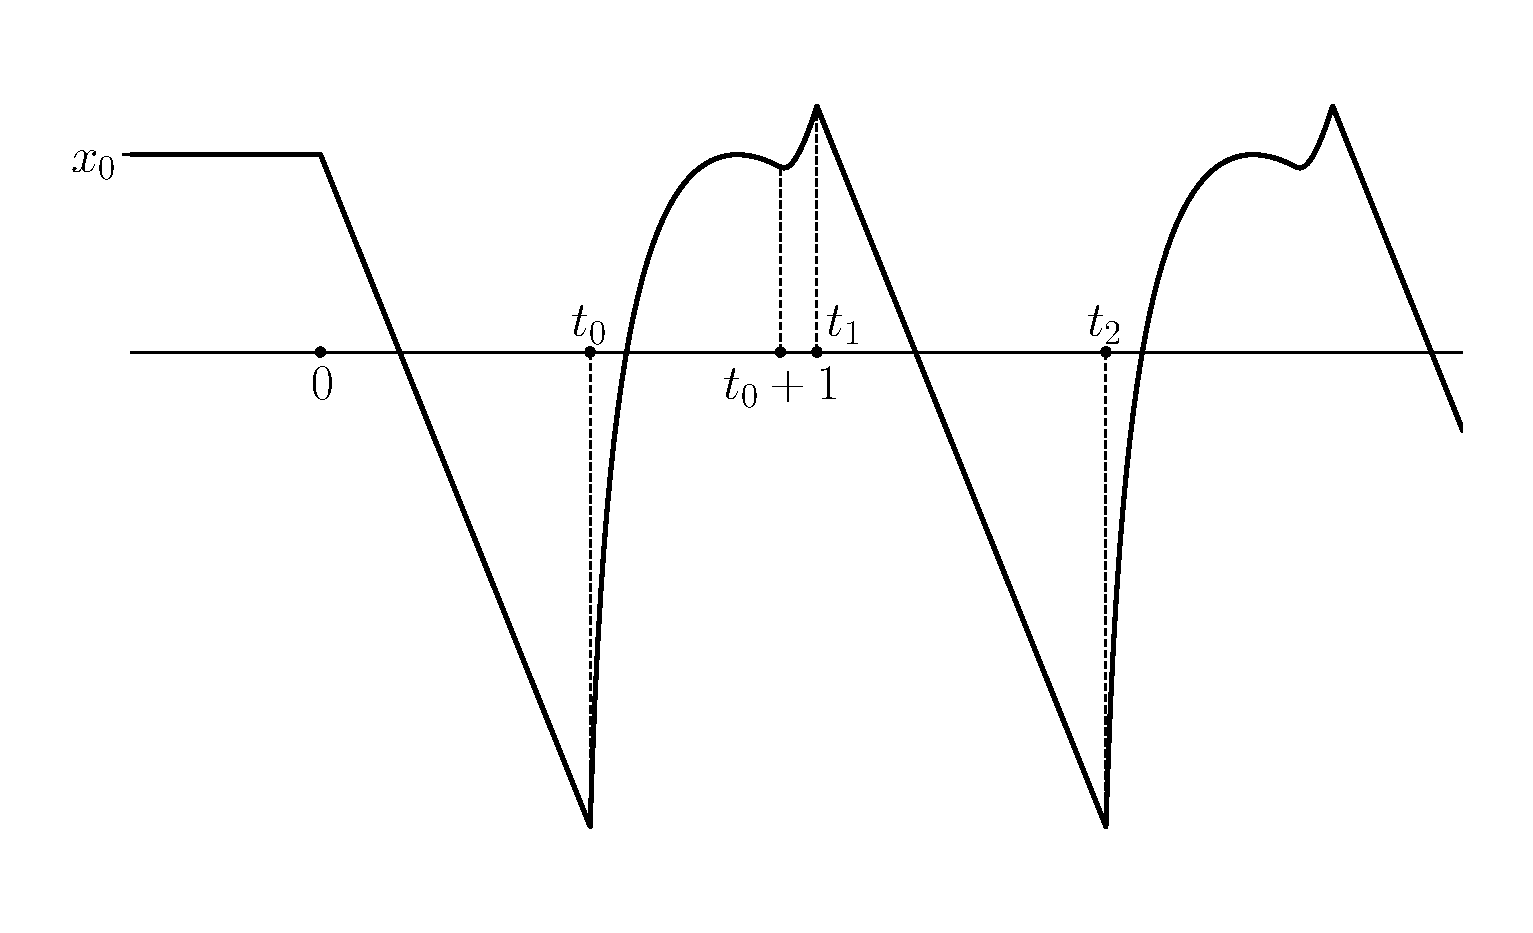
\includegraphics[width=0.7\textwidth]{x_star.eps}
	\captionof{figure}{Периодическое решение $x^{*}(t)$ уравнения \eqref{eq:intro:MG_rele}.}
	\label{fig:intro:x_star:ch1}
\end{figure}

Основной результат главы формулируется следующим образом.
	
\bigskip

\textbf{Теорема.} Пусть параметры $\alpha > \beta > 0$ удовлетворяют условиям \eqref{eq:intro:cond_alpha1}, \eqref{eq:intro:cond_alpha2}, $\alpha > \beta e^{\beta}$. Тогда существуют такие значения параметров $\sigma_0, p, q$ и такое достаточно большое $\gamma_0$, что при всех $\gamma > \gamma_0$ уравнение \eqref{eq:intro:MG_x} с начальной функцией $\varphi$ из множества \eqref{eq:intro:init_set} обладает периодическим решением $x^*_\gamma(t, \varphi)$ периода $T_{\gamma, \varphi}$ с асимптотикой
\footnotesize
\begin{equation}
	\label{eq:intro:sol_x*gamma}
	x^*_\gamma(t, \varphi)= 
	\begin{cases}
		- \beta t + O(\gamma^{-1} e^{-\beta \delta \gamma}), & t\in[-\sigma_0, 1 - \delta],\\
		-\beta + \frac{1}{\gamma} w_0(\tau)|_{\tau=(t - 1)\gamma} + O(\gamma^{-2\nu}), & t \in [1 - \delta,1 + \delta]\\
		- \beta t + \ln(\alpha e^{\beta}(t - 1) + 1) + O(\gamma^{-2\nu}) & t\in[1 + \delta, 2]\\
		- \beta t + \ln(\frac{\alpha^2}{2}e^{2 \beta}(t - 2)^2 + \alpha e^{\beta}(t - 1) + 1) + O(\gamma^{-2\nu}) & t \in [2, t_1 - \delta]\\
		- \beta t_1 + \ln(\eta)+\frac{1}{\gamma} w_1(\tau)|_{\tau=(t - t_1)\gamma} + O(\gamma^{-2\nu}) & t\in[t_1 - \delta, t_1  +\delta]\\
		- \beta t + \ln(\eta) + O(\gamma^{-2\nu}) & t \in [t_1 + \delta, t_2 - \delta]
	\end{cases}
\end{equation}
\normalsize
%
Данное решение удовлетворяет предельным равенствам 
%
\begin{equation}
	\label{eq:intro:lim_x*}
	\lim_{\gamma\to+\infty}\max_{0\leqslant t\leqslant T_{\gamma, \varphi}}|x_{\gamma}^*(t, \phi)-x^*(t)|=0,\quad \lim_{\gamma\to+\infty}T_{\gamma, \varphi} = T.
\end{equation}
Все остатки и пределы равномерны по $\varphi \in S$ и $t$ из соответствующих промежутков.

\bigskip
Во второй главе рассматривается полносвязная сеть релейных осцилляторов Мэки--Гласса, описываемая системой \eqref{eq:intro:mg_full_renormed}. Будем искать решение в виде дискретной бегущей волны. После подстановки $u_j(t) = u(t + j\Delta)$ получим вспомогательное уравнение \eqref{eq:intro:mg_auxiliary}.

Упорядочим множество запаздываний вспомогательного уравнения $\{1, \Delta, 2\Delta, \ldots, m\Delta\}$: пусть $\tau_0 \leq \tau_1 \leq \ldots \leq \tau_m$, где множество $\{\tau_j\}$ совпадает с множеством запаздываний. Затем отнормируем время так, чтобы наименьшее запаздывание стало равным единице. Получим уравнение 
\begin{equation}
	\label{eq:intro:mg_relay_w}
	\dot{u}=-\beta u+\alpha F(w(t)), \text{ где } w(t) = \sum\limits_{s = 0}^m u(t - \tau_s).
\end{equation}
%
Определим множество $S$ начальных функций на промежутке длины наибольшего запаздывания: 
%
\begin{equation}
	\label{eq:intro:mg_init_set}
	S = \{\varphi\in C[-\tau_{m},0]:\  \varphi(t)>1 \text{ при } t\in[-\tau_{m},0),\ \varphi(0)=u_0 > 1\}.
\end{equation}
%
Введём обозначения:
%
\begin{equation*}
	A = \sum_{i=0}^{m}e^{\beta \tau_{i}}=e^\beta+e^{\beta \tau_1}+\ldots+e^{\beta \tau_{m}},
\end{equation*}
\begin{equation*}
	\tau_* = \min\{2,\tau_1\}=\left\lbrace\begin{array}{cl}
		\min\{2,1/\Delta\}, & \text{ если } \Delta < 1,
		\\
		\min\{2,\Delta\}, & \text{ если } \Delta > 1,
	\end{array}\right.
\end{equation*}
\begin{equation*}
	s_* = t_1-t_0.
\end{equation*}
%
Для вспомогательного уравнения \eqref{eq:intro:mg_relay_w} верна следующая теорема.

\textbf{Теорема.} Пусть параметры $\alpha, \beta$ и величина $\tau_*$ удовлетворяют ограничениям

\begin{equation}
	\label{eq:intro:cond_thm1}
	\frac{\alpha}{\beta}e^{\beta}\left(\ln\left(\frac{\beta}{\alpha}\right)+1\right) < 1,
	\quad
	\alpha > \beta.
\end{equation}
%
\begin{equation}
	\label{eq:intro:cond_thm2}
	e^{\beta \tau_*}-1 \leqslant \alpha e^\beta(\tau_*-1)
	\quad\text{или}\quad
	0 < \frac{1}{\beta}\ln\frac{\alpha}{\beta}\leqslant\tau_*-1,
\end{equation}
%
\begin{equation}
	\label{eq:intro:cond_th_w>1_t_1+1}
	e^{-\beta s_*}(e^{-\beta}+\alpha s_*)>1
\end{equation}
%
\begin{equation}
	\label{eq:intro:cond_hair_hair_01}
	\frac{\alpha^2}{2}e^\beta(s_*-1)^2+\alpha s_*>\frac{e^{\beta \tau_k}-1}{\sum_{i=0}^{k-1}e^{\beta \tau_i}},\text{ если } s_*\leqslant \tau_k-\tau_{k-1},\quad k=1,\ldots,m,
\end{equation}
%
\begin{equation}
	\label{eq:intro:cond_hair_hair_02}
	\frac{\alpha^2}{2}e^\beta(s_*-1)^2+\alpha s_*>\frac{e^{\beta (s_*+\tau_{k-1})}-1}{\sum_{i=0}^{k-1}e^{\beta \tau_i}},\text{ если } s_* > \tau_k-\tau_{k-1},\quad k=1,\ldots,m,
\end{equation}
%
\begin{equation}
	\label{eq:intro:cond_hair_hair_1}
	\frac{\alpha^2}{2}e^\beta( s_*-1)^2+\alpha s_*>\frac{(e^{\beta s_*}-\alpha s_*)e^{\beta \tau_k}-1}{\sum_{i=0}^{k-1}e^{\beta \tau_i}},\quad k=1,\ldots,m.
\end{equation}
Тогда решение уравнения \eqref{eq:mg_relay_w} при любой начальной функции из множества \eqref{eq:mg_init_set} совпадает с одной и той же периодической функцией. Назовём эту функцию $u_*$, а её период $T$. Справедливо следующее.

1. Функция $u_*(t)$ обладает наименьшим числом переключений на периоде: $t_0$, $t_0+1$, $t_1$. При этом 
%
\begin{equation*}
	t_0=\frac{1}{\beta}\ln(u_0 A),
\end{equation*}
\begin{equation}
	e^{\beta s_*} - 1=\alpha e^{\beta}(s_* - 1), \quad s_* \in (1, \tau_*).
\end{equation}

2. Функция $u_*(t)$ и период $T$ имеют следующий явный вид: 
%
\small
\begin{equation}
	\label{eq:intro:u_star}
	u_*(t)=
	\begin{cases}
		u_0 e^{-\beta t}(\alpha A(t-t_0)+1) & \text{ при } t\in[t_0,t_0+1].
		\\
		u_0 e^{-\beta t}\left(\frac{\alpha^2}{2}Ae^{\beta}(t-t_0-1)^2+\alpha A(t-t_0)+1\right) & \text{ при } t\in[t_0+1,t_1],
		\\
		u_0 e^{-\beta t}\left(\frac{\alpha^2}{2}Ae^{\beta}(t_1-t_0-1)^2+\alpha A(t_1-t_0)+1\right) & \text{ при } t\in[t_1,t_0+T].
	\end{cases}
\end{equation}
\normalsize
%
\[
u_*(t + T) \equiv u_*(t),
\]
%
\begin{equation}
	\label{eq:intro:mg_period_T}
	T = \dfrac{1}{\beta}\ln\left( \frac{\alpha^2}{2}Ae^{\beta}(t_1-t_0-1)^2+\alpha A(t_1-t_0)+1\right). 
\end{equation}
%
Схематичный график функции $u_*$ изображён на рисунке \ref{fig:intro:u_star}.
%
\begin{figure}[h]
	\centering
	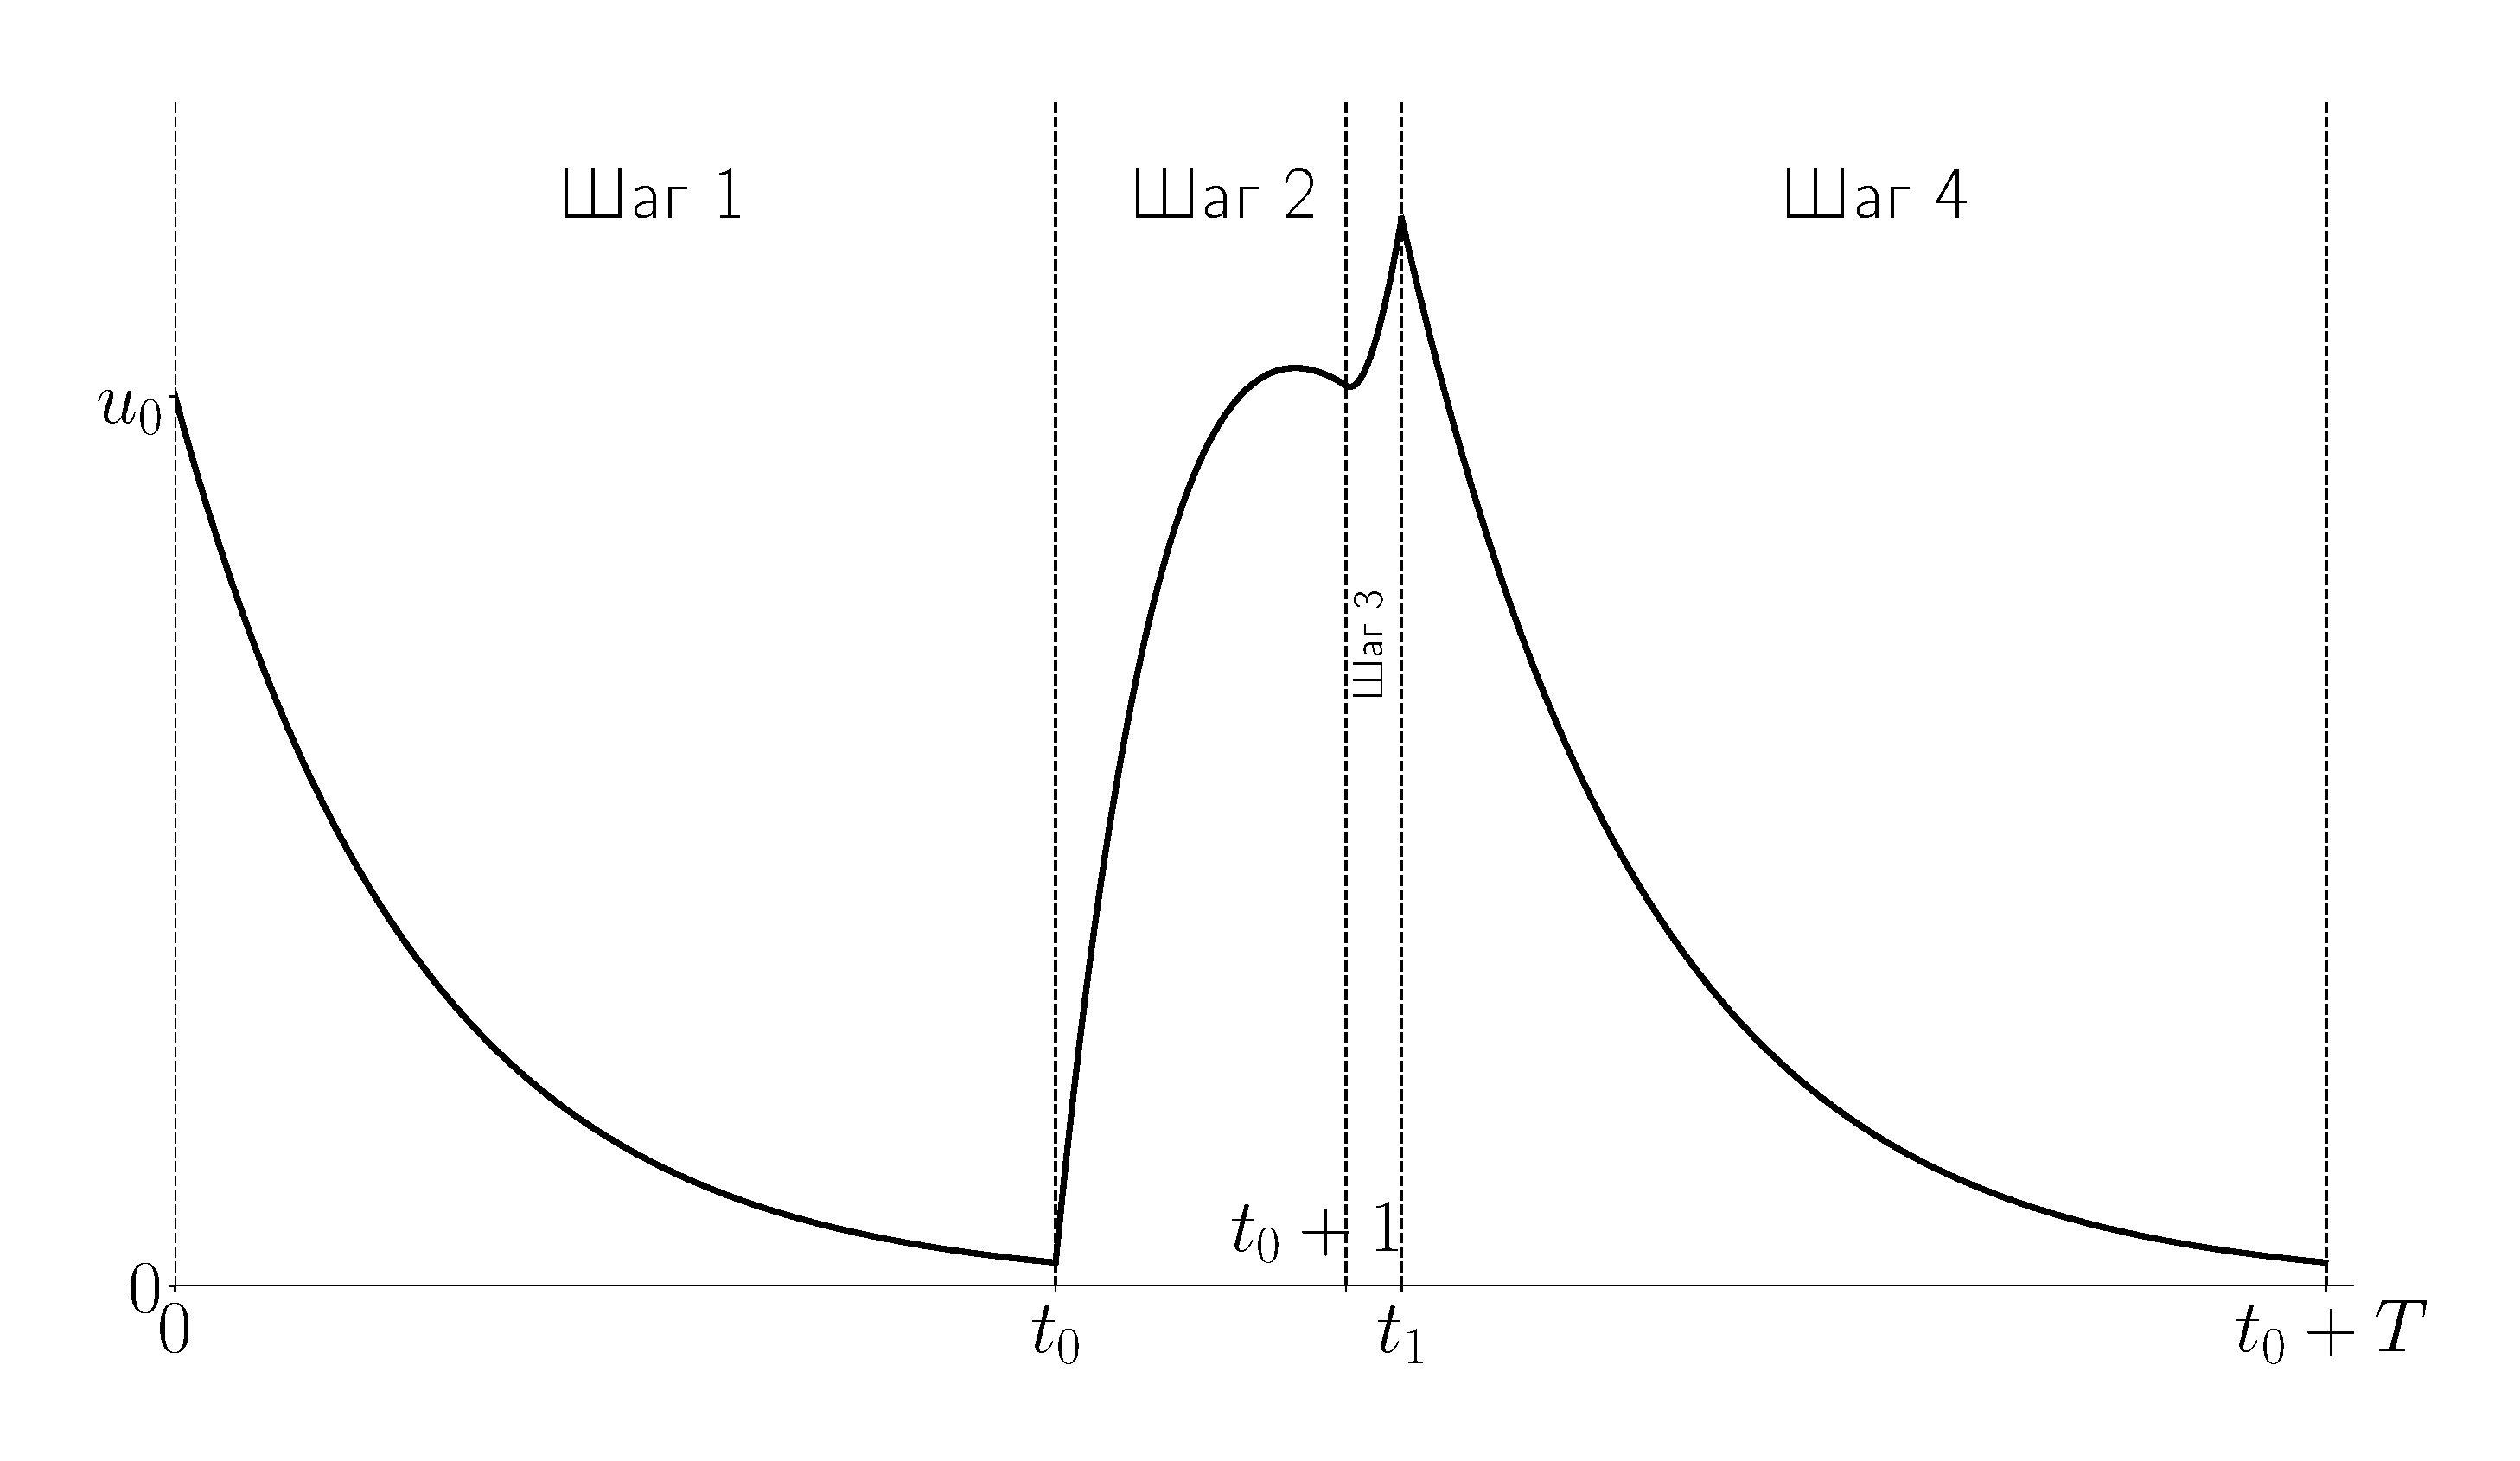
\includegraphics[width=0.7\textwidth]{u_star.eps}
	\caption{Функция $u_*(t)$, определённая на периоде $[t_0, t_0 + T]$ уравнением \eqref{eq:intro:u_star}.}
	\label{fig:intro:u_star}
\end{figure}

Для существования дискретной бегущей волны нужно проверить, что при некотором $\Delta$ период решения вспомогательного уравнения кратен $\Delta (m + 1)$, где $(m + 1)$ --- число уравнений в системе, т.е. для некоторого $p \in \mathbb{N}$ выполнено
\begin{equation}
	\label{eq:intro:period_eq}
	pT = \Delta (m + 1).
\end{equation}

Верна теорема.

\textbf{Теорема.} Для произвольных 
%
\begin{equation}
	\label{eq:intro:constraints_parameters_final}
	\beta > 0, \alpha \geq e^{\beta\left(1 + \frac{1}{e^{\beta}}\right)} - 1
\end{equation}
%
найдётся $\Delta > 1$, при котором набор параметров $\alpha, \beta, \Delta$ удовлетворяет уравнению \eqref{eq:intro:period_eq} и условиям \eqref{eq:intro:cond_thm1}, \eqref{eq:intro:cond_thm2}, \eqref{eq:intro:cond_th_w>1_t_1+1}, \eqref{eq:intro:cond_hair_hair_01}, \eqref{eq:intro:cond_hair_hair_02}, \eqref{eq:intro:cond_hair_hair_1}.

Из справедливости данной теоремы сразу следует существование решения в виде дискретной бегущей волны у уравнения \eqref{eq:intro:mg_full_renormed} при данных ограничениях на параметры. Численные эксперименты показывают, что решение является устойчивым; более того, результаты экспериментов позволяют предположить глобальную притягиваемость решений данного вида.

\bigskip

В третьей главе рассматривается полносвязная сеть, состоящая из $N = n + m$ релейных осцилляторов Мэки--Гласса, описываемая системой \eqref{eq:intro:mg_full_renormed_delta}. Будем искать решение, описывающее режим двухкластерной синхронизации. После подстановки \eqref{eq:intro:cluster} получим вспомогательное уравнение \eqref{eq:intro:system_uv}.

После замен
\begin{equation}
	\label{eq:intro:tilde_change}
	\tilde{u}(t) = u(t - 1) + \delta (m - 1) u + \delta n v, \quad \tilde{v}(t) = v(t - 1) + \delta m u + \delta (n - 1) v,
\end{equation}
%
и последующей экспоненциальной подстановки
\begin{equation}
	\label{eq:intro:exp_change}
	\tilde{u} = e^x, \quad \tilde{v} = e^y
\end{equation}
%
система \eqref{eq:intro:system_uv} примет вид
%
\begin{equation}
	\label{eq:intro:system_cluster_main}
	\begin{cases}
		\dot{x} = -\beta + \alpha \left(e^{x(t - 1) - x} G(x(t - 1)) + \delta (m - 1) G(x) + \delta n e^{y - x} G(y)\right),\\
		\dot{y} = -\beta + \alpha \left(e^{y(t - 1) - y} G(y(t - 1)) + \delta m e^{x - y} G(x) + \delta (n - 1) G(y)\right),
	\end{cases}
\end{equation}
где $G(x) = e^{-x} \, F(e^x)$.

Данная замена корректна в смысле следующей теоремы.

\textbf{Теорема.} Пусть $(x, y)$ --- $T$-периодическое решение системы \eqref{eq:intro:system_cluster_main}. Тогда существуют $T$-периодические функции $u, v$, однозначно определяемые соотношениями \eqref{eq:intro:tilde_change}, \eqref{eq:intro:exp_change}, которые являются решением системы \eqref{eq:intro:system_uv}.

Как и в предыдущей части диссертации, будем исследовать предельный при $\gamma \to +\infty$ объект. Подменим функцию $G$ предельной, т.~е. в уравнении \eqref{eq:intro:system_cluster_main} будем считать, что функция $G$ имеет вид 
\begin{equation}
	\label{eq:intro:relay_G_tilde}
	G(x) = \lim\limits_{\gamma \to +\infty} \dfrac{1}{1 + e^{\gamma x}} = 
	\begin{cases}
		0, & x > 0,\\
		1/2, & x = 0,\\
		1, & x < 0.
	\end{cases}
\end{equation}
%
В этом случае правая часть релейной системы \eqref{eq:intro:system_cluster_main} имеет разрыв в правой части при $x = 0$ и при $y = 0$. Анализ системы показывает, что её решение при достижении одной из прямых разрыва может продолжаться только вдоль этой прямой (трансверсальное пересечение прямой разрыва оказывается невозможным). В связи с этим будем искать обобщённое решение системы: будем полагать, что при $x \neq 0$ функция $G$ описывается уравнением \eqref{eq:intro:relay_G_tilde}, а в случае $x = 0$ принимает то значение из промежутка $(0, 1)$, при котором решение $(x, y)$ продолжается вдоль прямой $x = 0$; аналогично определяется движение по прямой $y = 0$. В такой постановке данный метод соответствует методу эквивалентного управления \cite{Utkin1981}, однако в силу специфики данной системы, такое доопределение оказывается эквивалентным другим вариантам обобщения понятия решения системы ДУ, приведённым в \cite{Filippov1988}.


Определим на множестве $[-1, 0]$ семейство пар начальных функций. Фиксируем $x_0 > y_0 > 0$.
\small
\begin{equation}
	\label{eq:intro:initial_set}
	S = \left\{\phi, \psi \in C[-1, 0] \,|\, \phi(t) > 0, \psi(t) > 0, x_0 = \phi(0), y_0 = \psi(0)\right\}.
\end{equation}
\normalsize

Справедлива следующая теорема.

\bigskip

\textbf{Теорема.}
	Пусть 
	%
	\begin{equation}
		\label{eq:intro:constraint_1}
		x_0 - y_0 < \ln \dfrac{e^{2\beta}(n - \delta(n - 1)) - ne^{\beta} + \delta n(n - 1)}{\delta (n - 1)^2},
	\end{equation}
	\begin{equation}
		\label{eq:intro:constraint_2}
		\beta < \alpha \delta (m - 1), \quad \beta < \alpha \delta (n - 1),
	\end{equation}
	\small
	\begin{equation}
		\label{eq:intro:constraint_3}
		e^{\beta} \cdot \dfrac{n - \delta(n - 1)}{\delta (n - 1)^2} > \dfrac{1}{n - 1} + \dfrac{1}{\delta(m - 1)}, \quad
		e^{\beta} \cdot \dfrac{m - \delta(m - 1)}{\delta (m - 1)^2} > \dfrac{1}{\delta(n - 1)} + \dfrac{1}{m - 1}.
	\end{equation}
	\normalsize
	
	При ограничениях \eqref{eq:intro:constraint_1}, \eqref{eq:intro:constraint_2}, \eqref{eq:intro:constraint_3}  и произвольных начальных функциях из множества \eqref{eq:intro:initial_set} релейное уравнение \eqref{eq:intro:system_cluster_main} имеет обобщённое решение, описываемое формулами
	%
	\small
	\begin{equation}
		\label{eq:intro:step1_solution}
		\begin{cases}
			x = x_0 - \beta t,\\
			y = y_0 - \beta t
		\end{cases}
		\text{при } t \in [0, t_0], \text{ где } t_0 = \dfrac{y_0}{\beta};
	\end{equation}
	%
	\begin{equation}
		\label{eq:intro:step2_solution}
		\begin{cases}
			x = x_0 - \beta t + \ln\left(1 + \frac{n}{n - 1} e^{-x_0 + \beta t_0}  (e^{\beta  (t - t_0)} - 1)\right),\\
			y = 0
		\end{cases}
		\text{при } t \in [t_0, t_0 + 1];
	\end{equation}
	%
	\begin{multline}
		\label{eq:intro:step3_solution}
		\begin{cases}
			x = -\beta t + \ln\left(\exp(x(t_{2i} + 1) + \beta (t_{2i} + 1)) + \frac{n (\delta(n - 1) - 1)}{\delta (n - 1)^2} (e^{\beta t} - \exp(\beta (t_{2i} + 1)))\right)
			,\\
			y = 0
		\end{cases}\\
		\text{при } t \in [t_{2i} + 1, t_{2i + 1}];
	\end{multline}
	%
	\begin{multline}
		\label{eq:intro:step4_solution}
		\begin{cases}
			x = 0,\\
			y = -\beta t + \ln\left(\exp(\beta t_{2i + 1}) + \left(\frac{1}{\delta(n - 1)} + \frac{m}{m - 1}\right) (e^{\beta t} - \exp(\beta t_{2i + 1}))\right)
		\end{cases}\\
		\text{при } t \in [t_{2i + 1}, t_{2i} + 2];
	\end{multline}
	%
	\begin{multline}
		\label{eq:intro:step5_solution}
		\begin{cases}
			x = 0,\\
			y = -\beta t + \ln\left(\exp(y(t_{2i} + 2) + \beta (t_{2i} + 2)) + \left(\frac{\delta(n - 1) - 1}{\delta^2 (n - 1)^2} + \frac{m}{m - 1}\right) (e^{\beta t} - \exp(\beta (t_{2i} + 2)))\right)
		\end{cases}\\
		\text{при } t \in [t_{2i} + 2, t_{2i + 1} + 1];
	\end{multline}
	%
	\begin{multline}
		\label{eq:intro:step6_solution}
		\begin{cases}
			x = 0,\\
			y = -\beta t + \ln\left(\exp(y(t_{2i + 1} + 1) + \beta(t_{2i + 1} + 1)) + \frac{m (\delta (m - 1) - 1)}{\delta (m - 1)^2} (e^{\beta t} - \exp(\beta (t_{2i + 1} + 1))) \right)
		\end{cases}\\
		\text{при } t \in [t_{2i + 1} + 1, t_{2i + 2}];
	\end{multline}
	%
	\begin{multline}
		\label{eq:intro:step7_solution}
		\begin{cases}
			x = -\beta t + \ln\left(\exp(\beta t_{2i + 2}) + \left(\frac{1}{\delta(m - 1)} + \frac{n}{n - 1}\right) (e^{\beta t} - \exp(\beta t_{2i + 2}))\right),\\
			y = 0
		\end{cases}\\
		\text{при } t \in [t_{2i + 2}, t_{2i + 1} + 2];
	\end{multline}
	%
	\begin{multline}
		\label{eq:intro:step8_solution}
		\begin{cases}
			x = -\beta t + \ln\left(\exp(x(t_{2i + 1} + 2) + \beta (t_{2i + 1} + 2)) + \left(\frac{\delta(m - 1) - 1}{\delta^2 (m - 1)^2} + \frac{n}{n - 1}\right) (e^{\beta t} - \exp(\beta (t_{2i + 1} + 2)))\right),\\
			y = 0
		\end{cases}\\
		\text{при } t \in [t_{2i + 1} + 2, t_{2i + 2} + 1];
	\end{multline}
	%
	\begin{multline}
		\label{eq:intro:step9_solution}
		\begin{cases}
			x = -\beta t + \ln\left(\exp(y(t_{2i + 2} + 1) + \beta(t_{2i + 2} + 1)) + \frac{n (\delta(n - 1) - 1)}{\delta (n - 1)^2} (e^{\beta t} - \exp(\beta (t_{2i + 2} + 1))) \right),\\
			y = 0
		\end{cases}\\
		\text{при } t \in [t_{2i + 2} + 1, t_{2i + 3}].
	\end{multline}
	\normalsize
	
	Здесь $i \geqslant 0$ --- целое число. Каждый момент времени $t_{2i + 1}$ определяется как корень уравнения $x = 0$, где функция $x(t)$ задаётся уравнением \eqref{eq:intro:step3_solution}. Каждый момент времени $t_{2i + 2}$ определяется как корень уравнения $y = 0$, где функция $y(t)$ определяется уравнением \eqref{eq:intro:step6_solution}. Для всех $i \geqslant 0$ верно, что $t_{i + 1} \in (t_i + 1, t_i + 2)$.


\begin{figure}[!ht]
	\centering
	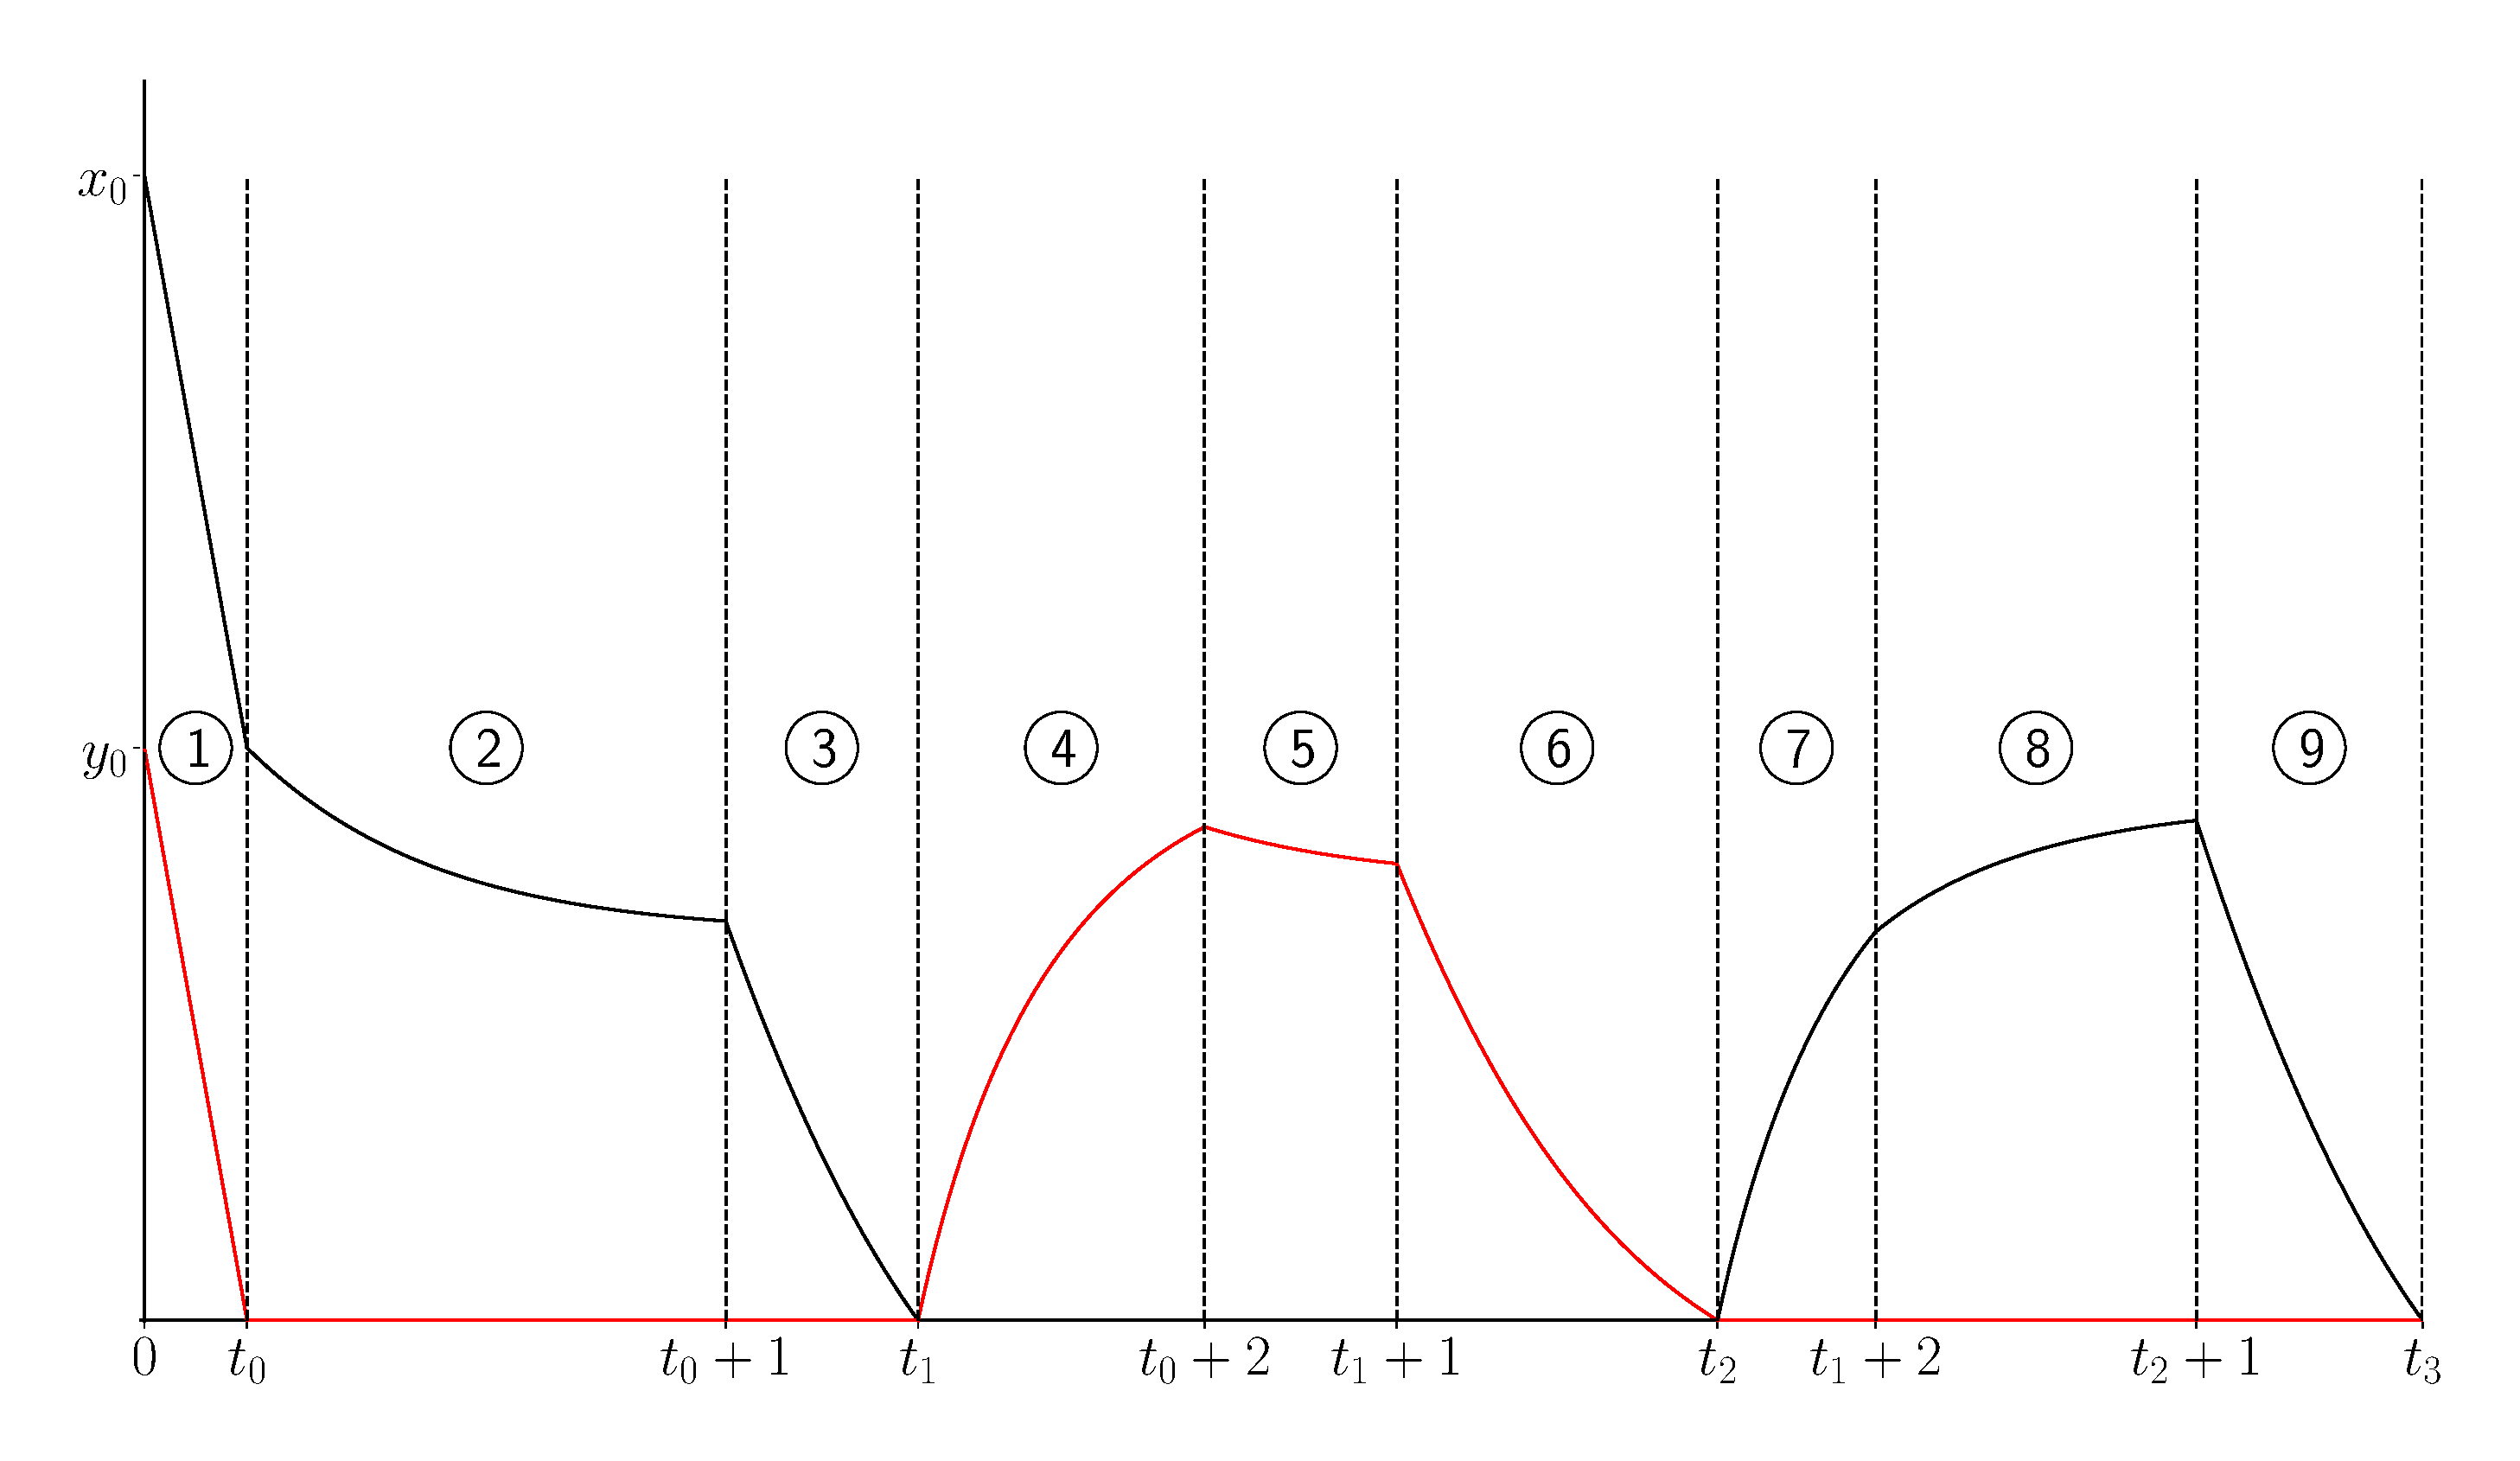
\includegraphics[width=\textwidth]{cluster_step_by_step.eps}
	\caption{Обобщённое решение релейной системы \eqref{eq:intro:system_cluster_main}, построенное методом шагов. Чёрная линия --- компонента решения $x$, красная линия --- компонента решения $y$. Числа в кругах означают номер шага построения.}
	\label{fig:intro:cluster_step_by_step}
\end{figure}

Основным результатом третьей главы является следующая теорема.

\textbf{Теорема.} При ограничениях \eqref{eq:intro:constraint_1}, \eqref{eq:intro:constraint_2}, \eqref{eq:intro:constraint_3} релейная система \eqref{eq:intro:system_cluster_main} имеет периодическое решение, описываемое на периоде $[t_1, t_3]$ формулами \eqref{eq:intro:step4_solution} -- \eqref{eq:intro:step9_solution}.



